\documentclass[pdflatex,onecolumn,sn-mathphys-num]{sn-jnl}

% =========================================================
% Packages
% =========================================================
\usepackage{graphicx}
\usepackage{multirow}
\usepackage{amsmath,amssymb,amsfonts}
\usepackage{amsthm}
\usepackage[title]{appendix}
\usepackage{xcolor}
\usepackage{textcomp}
\usepackage{manyfoot}
\usepackage{booktabs}
\usepackage{algorithm}
\usepackage{algorithmicx}
\usepackage{algpseudocode}
\usepackage{listings}
\usepackage{microtype}
\usepackage{float}
\usepackage{placeins}

% =========================================================
% Layout
% =========================================================
\setlength{\jot}{6pt}
\emergencystretch=3em
\hfuzz=2pt
\vfuzz=2pt
\hbadness=10000
\vbadness=10000
\raggedbottom

\hypersetup{hypertexnames=false}

% =========================================================
% Footnote rule
% =========================================================
\makeatletter
\renewcommand{\footnoterule}{%
    \kern -3pt
    \hrule width \textwidth height 0.4pt
    \kern 4pt
}
\makeatother

% =========================================================
% Document
% =========================================================
\usepackage{longtable}
\makeatletter
% Longtable captions must use the same "Table N<space>text" prefix as the ordinary
% \@tablecaption of sn-jnl.cls.  The longtable default inserts a colon, and the
% preamble previously passed longtable's second argument (the short-list entry, #2)
% where the caption text is expected, which dropped the "Table N" prefix altogether.
% Here the numbering comes from #1 and the caption text from #3, and the text is
% centred across as many lines as it needs.
\renewcommand\LT@makecaption[3]{%
  \LT@mcol\LT@cols c{\hbox to\z@{\hss\parbox[t]\LTcapwidth{%
    \reset@font\centering
    #1{#2\hskip2mm}#3%
    \endgraf\vskip\baselineskip}%
  \hss}}}
\makeatother
\begin{document}

% =========================================================
% Title
% =========================================================
\title[LSCBO Scheduler]{L\'{e}vy-Assisted Coyote-Badger Optimization with Pareto-Safe Pair Reassignment for Cloud Task Scheduling}

% =========================================================
% Authors
% =========================================================
\author[a]{\fnm{Yarui} \sur{Yuan}\textsuperscript{*}}
\author[a]{\fnm{Yubo} \sur{Wang}}
\author[a]{\fnm{Chengshu} \sur{Zhu}}
\author[b]{\fnm{Zhanhui} \sur{Li}}

% =========================================================
% Affiliation
% =========================================================
\affil[a]{
    \orgname{Chengyi College, Jimei University},
    \orgaddress{\city{Xiamen}, \country{China}}
}
\affil[b]{
    \orgname{Tencent CSIG},
    \orgaddress{\city{Hangzhou}, \country{China}}
}

% =========================================================
% Corresponding author footnote
% =========================================================
\begingroup
\renewcommand{\thefootnote}{*}
\begin{NoHyper}
\footnotetext{%
Corresponding author.\\
E-mail address: yaruiyuan@163.com
}
\end{NoHyper}
\endgroup

% =========================================================
% Abstract
% =========================================================
\abstract{Effective task scheduling in cloud computing requires the simultaneous consideration of multiple costs, including makespan, energy consumption, execution cost, and load imbalance. However, optimizing a weighted scalar objective may conceal deterioration in individual cost criteria. To address this issue, this study proposes LSCBO, a Lévy-assisted Coyote-Badger Optimization framework with Pareto-safe pair reassignment for multi-cost cloud task scheduling. LSCBO integrates a continuous search core based on Coyote-Badger Optimization, an auxiliary heavy-tailed Lévy Flight mechanism, and a discrete Pareto-safe pair-reassignment operator for decoded task-to-VM assignments. A Greedy-LPT schedule provides a shared warm start and fixed reference denominators for multi-cost normalization. To evaluate the proposed method, two experimental series are conducted. First, experiments on 29 official CEC2017 benchmark functions show that LSCBO achieves the lowest average Friedman rank of 1.690 among nine meta-heuristic optimizers. Second, experiments on 150 paired analytical cloud scheduling instances covering multiple task scales show a mean reduction of 1.65\% in the normalized multi-cost objective, with a 95\% bootstrap confidence interval of 1.47\%–1.84\%, while load imbalance is reduced by 5.65\%–6.81\% across task scales relative to Greedy-LPT. Ablation results indicate that the observed improvement in the cloud scheduling experiments is primarily associated with the Pareto-safe pair-reassignment operator. These results support the use of LSCBO for multi-cost refinement under the analytical scheduling model while highlighting the need for further validation in larger and more diverse cloud environments.}

% =========================================================
% Keywords
% =========================================================
\keywords{Cloud task scheduling; Coyote-Badger Optimization; L\'{e}vy flight; Pareto-safe pair reassignment; Multi-cost optimization}

% =========================================================
% Generate title + abstract + keywords
% =========================================================
\maketitle

% =========================================================
% 1 Introduction
% =========================================================

\section{Introduction}

Cloud computing has become an important computing paradigm for delivering scalable computational resources through virtualized infrastructures~\cite{Armbrust2010,Buyya2009}. Within cloud datacenters, task scheduling determines how computational workloads are assigned to heterogeneous virtual machines (VMs) with different processing capacities, thereby affecting makespan, energy consumption, execution cost, and resource utilization~\cite{Coffman1976,Braun2001,Etminani2007}. When task workloads and VM processing capacities are known in advance, the scheduling problem can be formulated as an assignment problem in which each task must be allocated to one available VM. Although this formulation is conceptually simple, the resulting search space grows rapidly with the number of tasks and VMs. More importantly, practical scheduling decisions usually involve multiple performance criteria rather than a single optimization target. An effective scheduling method therefore needs not only to explore a large combinatorial search space but also to manage the trade-offs among different cost criteria under a limited computational budget.

Population-based meta-heuristic algorithms provide a flexible approach to such computationally difficult optimization problems. Particle Swarm Optimization (PSO) and evolutionary algorithms have been widely applied to complex optimization problems because they do not require gradient information and can explore large search spaces through population-based candidate generation~\cite{Kennedy1995,Goldberg1989,Yang2014}. A range of continuous optimizers has subsequently been developed using different exploration and exploitation mechanisms. The Whale Optimization Algorithm (WOA) models the bubble-net hunting behavior of humpback whales~\cite{Mirjalili2016}, while the Grey Wolf Optimizer (GWO) uses a hierarchical hunting strategy to guide population evolution~\cite{Mirjalili2014}. The Dung Beetle Optimizer (DBO) introduces several behavior-inspired search strategies for global optimization~\cite{Xue2022}, and the Arithmetic Optimization Algorithm (AOA) employs arithmetic operators to control the balance between exploration and exploitation~\cite{Abualigah2021}. More recently, Coyote-Badger Optimization (CBO) has introduced a cooperative hunting-based population search framework~\cite{Khatab2025}. In cloud task scheduling, these continuous optimization mechanisms are commonly combined with problem-specific representations and search operators. Recent studies have further incorporated L\'{e}vy-flight perturbations, chaotic mappings, and hybrid optimization mechanisms to improve the exploration or refinement capability of meta-heuristic schedulers~\cite{Chintale2024,Sabipour2025,Zhu2025}.

Despite the flexibility of meta-heuristic optimization, two structural issues remain when continuous population-based search is applied to multi-cost cloud task scheduling. First, weighted scalarization provides a convenient basis for ranking candidate schedules, but an improvement in the aggregated objective does not necessarily prevent deterioration in individual criteria, such as makespan, energy consumption, execution cost, or load imbalance. Multi-objective methods such as NSGA-II and MOEA/D explicitly represent trade-offs among conflicting objectives~\cite{Deb2002,Zhang2007}, whereas a single deployable schedule may instead require a scalar preference together with constraints on individual criteria. Second, continuous search must ultimately be mapped to discrete task-to-VM assignments. With a floor- or rounding-based decoder, multiple continuous positions can produce the same assignment, creating piecewise-constant objective regions in which small continuous perturbations do not change the actual schedule. These two issues motivate a complementary strategy that retains the scalar objective for overall preference while introducing component-wise admissibility and a discrete neighborhood operator for direct assignment-level refinement.

To overcome these structural limitations, this study proposes LSCBO, a L\'{e}vy-assisted Coyote-Badger Optimization framework integrated with Pareto-safe pair reassignment for multi-cost cloud task scheduling. The proposed framework integrates continuous global exploration with assignment-level discrete refinement. Its continuous search core follows the searching, encircling, and attacking structure of CBO~\cite{Khatab2025} and is augmented with an auxiliary L\'{e}vy-flight mechanism to enhance long-range exploration~\cite{Mantegna1994}. Continuous candidates are decoded into feasible task-to-VM assignments, while a deterministic Greedy-LPT schedule provides both a common warm start and a fixed reference for normalizing the four scheduling criteria. After decoding, the Pareto-safe pair-reassignment operator directly explores the assignment neighborhood by exchanging pairs of tasks assigned to different VMs. A candidate exchange is accepted only when all four criteria---makespan, energy consumption, execution cost, and load imbalance---are non-worsening within a specified numerical tolerance and the weighted scalar objective is strictly improved. This acceptance rule separates component-wise admissibility from overall scalar preference and limits undesirable trade-offs during local refinement.

The main contributions of this study are summarized as follows:

\begin{itemize}
    \item A component-controlled LSCBO optimization framework: We integrate a CBO-based continuous search core, an auxiliary L\'{e}vy-flight exploration mechanism, direct task-to-VM decoding, and assignment-level pair reassignment into a unified continuous-to-discrete optimization architecture, bridging global exploration and discrete refinement under a controlled evaluation budget.

    \item A Pareto-safe pair-reassignment operator for local refinement: We design a scheduling-specific neighborhood operator that directly executes task exchanges across VMs. By coupling component-wise non-worsening admissibility conditions (for makespan, energy consumption, execution cost, and load imbalance) with strict scalar-objective preference, the operator achieves targeted local refinement while eliminating hidden trade-off deteriorations.

    \item A controlled empirical methodology for decoupled evaluation: We establish a rigorous experimental protocol that independently evaluates continuous optimizer performance (via CEC2017 benchmarks) and cloud scheduling efficacy (via matched ablations and sensitivity analyses). Furthermore, schedule executability is validated through a dedicated CloudSim Plus replay.

\end{itemize}


The remainder of this paper is organized as follows. Section 2 reviews related work on cloud task scheduling and hybrid meta-heuristics. Section 3 presents the mathematical model, the proposed LSCBO framework, and its computational complexity. Section 4 presents the empirical evaluation on both continuous benchmarks and cloud scheduling scenarios. Section 5 discusses the mechanism-level contributions, practical insights, and study limitations. Finally, Section 6 concludes the paper and outlines future research directions.

\section{Literature Review}\label{sec:literature}

Cloud scheduling combines general optimization procedures with a domain-specific assignment and cost model. Swarm methods such as PSO~\cite{Kennedy1995}, evolutionary methods such as GA~\cite{Goldberg1989}, and simulated annealing~\cite{Kirkpatrick1983} use different search mechanisms. For scheduling, the representation and evaluator determine how these mechanisms are translated into candidate assignments. The relevant literature is therefore organized around multi-cost models, scheduling adaptations, and local refinement.

\subsection{Multi-Cost Cloud Task Scheduling Models}

Deterministic dispatching rules provide computationally inexpensive assignments for heterogeneous resources. Min-Min and Max-Min use estimated completion times to select assignments~\cite{Etminani2007}, while FCFS follows task order. Such rules are useful baselines: whether additional optimization improves them depends on the workload, resource model, and evaluation criteria. In particular, a rule focused on completion time does not explicitly control every trade-off in a combined cost objective.

Multi-cost models extend completion-time evaluation with energy, execution cost, and load distribution. Multi-objective methods, including nondominated-sorting NSGA-II~\cite{Deb2002} and decomposition-based MOEA/D~\cite{Zhang2007}, seek sets of trade-off solutions; hybrid multi-objective workflow scheduling provides a related application~\cite{Verma2017}. Scalarized schedulers instead optimize one weighted objective for a selected preference profile. The present study uses this latter formulation and adds a component-wise condition to local moves, rather than constructing a Pareto front.

\subsection{Meta-Heuristic Schedulers for Cloud Task Assignment}

A continuous optimizer supplies candidate-update rules but does not by itself specify a cloud scheduler. Nature-inspired search designs include WOA~\cite{Mirjalili2016}, GWO~\cite{Mirjalili2014}, DBO~\cite{Xue2022}, and AOA~\cite{Abualigah2021}. Other examples are KOA~\cite{AbdelBasset2023}, SO~\cite{Hashim2022}, and SAO~\cite{Deng2023}. Further examples include POA~\cite{Trojovsky2022}, MPA~\cite{Faramarzi2020}, RSA~\cite{Abualigah2022}, and ARO~\cite{Wang2022}. Their scheduling adaptations must define how a candidate becomes a feasible assignment and how multiple costs are compared. This interface directly affects how the underlying search mechanism is applied to the scheduling problem and how its performance is evaluated.

Scheduling-specific examples include enhanced DBO~\cite{Xie2024}, the E-AVOA-TS fog--cloud scheduler~\cite{Ghafari2023}, ERTH for multi-cost cloud task scheduling~\cite{Qin2024}, and CEEO for IoT-generated cloud workloads~\cite{EbrahimiMood2025}. ERTH combines multiple elite policies and Bernoulli-map initialization with RTH to address multi-cost cloud task scheduling~\cite{Qin2024}. These studies illustrate how search modifications are connected to scheduling models. Their results are not direct comparators here because the present experiments use their own instances, normalization references, and evaluation budgets.

\subsection{Problem-Specific Hybridization and Local Search}

Hybridization is widespread in meta-heuristic cloud scheduling, although the contribution of an added operator varies. Examples include L\'{e}vy-enhanced Osprey Optimization~\cite{Chintale2024}, chaotic RIME with generalized quadratic interpolation and L\'{e}vy flight~\cite{Sabipour2025}, and hybrid SAO-RIME scheduling~\cite{Zhu2025}. A numerical method for generating L\'{e}vy-stable random variables is widely used in L\'{e}vy-flight implementations~\cite{Mantegna1994}. L\'{e}vy flights also form part of Cuckoo Search~\cite{YangDeb2009}.

A local assignment neighborhood provides a complementary way to refine a decoded schedule. In the memetic framework, a general search procedure is combined with problem-specific improvement~\cite{Moscato1989}. The task-pair neighborhood used here preserves the number of tasks on each participating VM but changes their processing loads. Requiring a scalar improvement together with component-wise admissibility distinguishes this operator from unrestricted objective-only exchange. A deterministic Greedy-LPT reference provides a demanding starting point against which this local contribution can be measured.

\subsection{Positioning and Comparison Boundary of LSCBO}

CBO models coyote--badger cooperation through searching, encircling, and attacking~\cite{Khatab2025}. It is distinct from the earlier Coyote Optimization Algorithm~\cite{Pierezan2018}. This study uses the paired three-stage structure as a search host and states the implemented adaptations explicitly. Methodological concerns about metaphor-based optimization motivate evaluating the resulting operators and their measured effects rather than treating the behavioral analogy as evidence of effectiveness~\cite{Sorensen2015}.

The empirical comparison includes CBO, PSO, GWO, WOA, AOA, and Greedy-LPT on identical task and VM instances. All population methods use the same decoder and deterministic first member. Ablation then separates the effects of continuous updates, L\'{e}vy proposals, the pair neighborhood, and the acceptance condition. This scope answers whether those mechanisms improve the stated scheduling model. Learning-based systems such as DeepRM~\cite{Mao2016} and Decima~\cite{Mao2019}, exact methods, and Pareto-front schedulers require different training, instance, or output protocols and remain outside this comparison.

% =========================================================
% 3 Research Methodology (complete source in this main file)
% =========================================================
\section{Research Methodology}\label{sec3}
LSCBO combines a continuous CBO-based search with task-pair refinement. The method proceeds from the scheduling model and fitness function to the search mechanisms, their cloud application, and computational cost.

\subsection{Cloud Task Scheduling Model}\label{sec:model}

\subsubsection{System Model and Assumptions}\label{sec:system}
The cloud datacenter provides $M$ heterogeneous virtual machines $V=\{VM_1,\ldots,VM_M\}$ to process $N$ independent tasks $T=\{T_1,\ldots,T_N\}$. Each task $T_i$ has a workload $W_i$, measured in million instructions (MI), and $VM_j$ provides an effective processing rate $\nu_j$, measured in million instructions per second (MIPS). This rate is the fixed capacity available to the assigned workload in the analytical model. The execution time of task $T_i$ on $VM_j$, in seconds, is
\begin{equation}\label{eq:exec_time}
t^{\mathrm{exec}}_{i,j}=\frac{W_i}{\nu_j}.
\end{equation}

All tasks are known before scheduling, as in static mapping of independent tasks~\cite{Braun2001}. The counts $N,M$ are positive integers, and all task lengths and VM rates are strictly positive. The binary variable $x_{i,j}=1$ means that task $T_i$ is assigned to $VM_j$, and $x_{i,j}=0$ otherwise. A feasible schedule $s$ assigns each task to exactly one available VM, so $\sum_{j=1}^{M}x_{i,j}=1$ for every task $i$.

The model has no precedence edges, communication delays, release dates, or per-task memory-fit constraints. It also excludes provisioning, dispatch, and context-switch overheads and changes in available capacity due to contention. VM completion times therefore represent accumulated processing loads. Equation~\eqref{eq:exec_time} also implies that a VM faster for one task is faster for all tasks, excluding task-specific accelerators and arbitrary task--machine execution-time interactions~\cite{Braun2001}. These assumptions define assignment feasibility but do not ensure that every schedule has a nonempty pair-exchange neighborhood. The optimization procedure below is specified for $N\geq2$; the single-task case is outside its stated algorithmic domain.

\subsubsection{Scheduling Criteria}\label{sec4}
\textbf{Makespan.}
Makespan and VM completion times are measured in seconds, with makespan denoting the time required to complete the assigned workload. For schedule $s$, the completion time of VM $j$ is the sum of its assigned processing times, $H_j(s)=\sum_{i=1}^{N}t^{\mathrm{exec}}_{i,j}x_{i,j}$, and the makespan is $H_{\mathrm{max}}(s)=\max_{1\leq j\leq M}H_j(s)$. An unused VM has zero completion time, whereas the makespan is positive under the assumptions above.

\begin{samepage}
\textbf{Analytical energy.}
The mean utilization over the makespan horizon is $u_j=H_j(s)/H_{\mathrm{max}}(s)\in[0,1]$. Let $P^{\mathrm{idle}}=\eta_P P^{\mathrm{max}}$, where $P^{\mathrm{max}}>0$ is in watts, $\eta_P\in[0,1]$, and $\gamma>0$ controls the utilization response. With $\kappa_t=3600$ seconds per hour, analytical energy in Wh is
\begin{equation}\label{eq:energy}
E(s)=\sum_{j=1}^{M}\left[P^{\mathrm{idle}}+(P^{\mathrm{max}}-P^{\mathrm{idle}})u_j^{\gamma}\right]\frac{H_{\mathrm{max}}(s)}{\kappa_t}.
\end{equation}
\end{samepage}

This mean-utilization proxy includes idle power from unused VMs. Its power parameters are analytical per-VM quantities, not calibrated measurements of physical-host electricity consumption. For nonlinear utilization response, evaluating power at the mean utilization is generally different from integrating instantaneous power. Equation~\eqref{eq:energy} therefore defines an analytical energy proxy rather than a time-resolved electricity measurement.

\begin{samepage}
\textbf{Execution cost.}
Let $\nu_{\mathrm{min}}\leq\nu_{\mathrm{max}}$ be the positive bounds of the configured processing-rate pool, with $\nu_{\mathrm{min}}\leq\nu_j\leq\nu_{\mathrm{max}}$ for every VM, and let $\epsilon_{\nu}>0$ be a denominator floor in MIPS. For $0\leq r_{\mathrm{min}}\leq r_{\mathrm{max}}$ in cost units per second, execution cost $C(s)$ is measured in cost units and uses the capacity-dependent rate $r_j$:
\begin{gather}
C(s)=\sum_{j=1}^{M}r_jH_j(s),\label{eq:cost}\\*
r_j=r_{\mathrm{min}}+(r_{\mathrm{max}}-r_{\mathrm{min}})\sqrt{\dfrac{\nu_j-\nu_{\mathrm{min}}}{\max\{\nu_{\mathrm{max}}-\nu_{\mathrm{min}},\epsilon_{\nu}\}}}.\label{eq:rate}
\end{gather}
\end{samepage}

The positive denominator floor keeps Eq.~\eqref{eq:rate} defined when the configured processing-rate bounds coincide. The rate is nondecreasing within the configured range but need not be proportional to capacity; it is synthetic rather than a fitted provider tariff.

\textbf{Load imbalance.}
Let $\overline{H}(s)=M^{-1}\sum_{j=1}^{M}H_j(s)$ denote the mean VM completion time. The dimensionless load-imbalance index is the population coefficient of variation of VM completion times,
\begin{equation}\label{eq:lbr}
\mathcal{I}(s)=\frac{\sqrt{\displaystyle M^{-1}\sum_{j=1}^{M}(H_j(s)-\overline{H}(s))^2}}{\overline{H}(s)}.
\end{equation}

The mean is positive under the stated task assumptions, and smaller values of $\mathcal{I}(s)$ indicate more even loads. The factor $M^{-1}$ corresponds to calculating variance over the full VM population.

Write the criterion vector as $\mathbf{f}(s)=(H_{\mathrm{max}}(s),E(s),C(s),\mathcal{I}(s))$, with all four components to be minimized. Its components are denoted by $f_{\mathrm{ms}}$, $f_{\mathrm{en}}$, $f_{\mathrm{cost}}$, and $f_{\mathrm{lb}}$, respectively, with index set $\mathcal{K}=\{\mathrm{ms},\mathrm{en},\mathrm{cost},\mathrm{lb}\}$.

\begin{samepage}
\subsubsection{Normalization and Fitness Function}\label{sec:fitness}
The deterministic Greedy-LPT schedule $s_g$ assigns tasks in decreasing instruction length to the VM with the earliest projected finish time and supplies the normalization reference. Equal-length tasks retain their original index order, and equal projected finish times select the smallest VM index. Choose $w_k\geq0$ with $\sum_k w_k=1$ and a positive floor $\varepsilon_k^{\mathrm{ref}}>0$ in each criterion\textquotesingle s units. Each fixed reference denominator $c_k>0$ has the same units as $f_k$, giving the dimensionless scalar fitness
\begin{gather}
c_k=\max\{f_k(s_g),\varepsilon_k^{\mathrm{ref}}\},\label{eq:reference}\\*
F(s)=\sum_{k\in\mathcal{K}}w_k\frac{f_k(s)}{c_k}.\label{eq:objective}
\end{gather}
\end{samepage}

The denominators are computed once per instance and held fixed across candidates and methods under the same comparison profile. If every reference value is at least its floor, $F(s_g)=1$.

Fitness $F$ is minimized directly without a reciprocal transformation, while local admissibility is tested separately. Weights and normalization influence the trade-offs expressed by a weighted sum~\cite{MarlerArora2010}; equal weights here apply to relative ratios, not equal physical savings. A lower $F$ need not improve every component, and finitely many weight profiles do not construct a complete Pareto front.

\subsection{LSCBO Algorithm Design}\label{sec:algorithm}

\subsubsection{Source CBO Mechanisms and a Planar Dynamic Adaptation}\label{sec:original_cbo}
The experimental comparator \emph{adapted CBO} denotes the core in Section~\ref{sec:enhancements} with auxiliary L\'{e}vy trials disabled. Its archived identifier \texttt{CBO} does not denote a reproduction of the source paper's static case studies.

Coyote-Badger Optimization organizes an even population of individual animals into coyote--badger couples~\cite{Khatab2025}. Let $n_{\mathrm{pop}}$ denote the even number of animals and let $p\in\{1,\ldots,n_{\mathrm{pop}}/2\}$ index a couple. For its coyote and badger positions $\mathbf{x}_p^c$ and $\mathbf{x}_p^b$, the prey midpoint is
\begin{equation}\label{eq:cbo_prey}
\mathbf{x}_p^{\mathrm{prey}}=\frac{\mathbf{x}_p^c+\mathbf{x}_p^b}{2}.
\end{equation}

The source divides $Z$ iterations into searching and encircling phases of $\lfloor Z/3\rfloor$ iterations each, followed by the remaining attacking iterations.

The source presents both dynamic and static variants. Dynamic searching applies
\begin{gather}
\mathbf{x}_p^{c,t+1}=\mathbf{x}_p^{c,t}\odot\left[\mathbf{1}+r_1\tanh(\mathbf{x}_p^{\mathrm{prey},t})\right],\label{eq:cbo_dynamic_search}\\*
\mathbf{x}_p^{b,t+1}=\mathbf{x}_p^{b,t}\odot\left[\mathbf{1}+r_2\tanh(\mathbf{x}_p^{\mathrm{prey},t})\right].\label{eq:cbo_badger_search}
\end{gather}

Here $t$ indexes searching iterations and $\odot$ denotes component-wise multiplication. The source gives $r_1,r_2\in[-0.5,0.5]$; the sampling law and frequency used in this study are specified with the implemented adaptation below. Searching clips positions to the domain and records visited positions without imposing greedy acceptance at every step. Static searching instead redraws animal positions in the search domain and takes the better animal as the prey.

Dynamic encircling rotates animal positions about the origin and retains fitness improvements. For $Z_{\mathrm{enc}}=\lfloor Z/3\rfloor>0$, set $\theta_t=2\pi t/Z_{\mathrm{enc}}$; if $Z_{\mathrm{enc}}=0$, skip this phase. The source's planar form is
\begin{gather}
\mathcal{R}_2(\theta_t)=
\begin{bmatrix}\cos\theta_t&-\sin\theta_t\\ \sin\theta_t&\cos\theta_t\end{bmatrix},\label{eq:rotation_matrix}\\*
\mathbf{x}^{t+1}=\mathcal{R}_2(\theta_t)\mathbf{x}^{t}.\label{eq:cbo_original_rotation}
\end{gather}

Equation~\eqref{eq:cbo_original_rotation} acts on a two-dimensional position; a higher-dimensional implementation requires a specified rotation operator. Dynamic attacking selects separate coyote and badger leaders and moves each animal to the midpoint between itself and its own subpopulation leader. The static variant rotates prey positions and subsequently samples inside the triangle formed by the three best prey positions. The original case studies use that static variant~\cite{Khatab2025}.

Algorithm~\ref{alg:original_dynamic_cbo} adapts the source's dynamic variant using planar rotation and leader selection for the scalar minimization objective $g$. On page~11 of the source paper, Eq.~(14) and line~9 of Algorithm~3 use the coyote position as the input to the badger rotation. Here, each animal rotates its own position; this convention is an explicit adaptation, without attributing an intended correction to the source authors. The source's static case studies are not reproduced here. Algorithm~\ref{alg:original_dynamic_cbo} illustrates the planar adaptation; the implementation evaluated in this study is specified in Sections~\ref{sec:enhancements} and~\ref{sec:cloud_procedure}, including initialization, higher-dimensional updates, sampling, retention, and evaluation rules.
\begin{algorithm}[p]
\caption{Planar adaptation of dynamic CBO~\cite{Khatab2025}}\label{alg:original_dynamic_cbo}
\small
\begin{algorithmic}[1]
\Statex \textbf{Input:} scalar objective $g$ to minimize; planar bounds $\boldsymbol{\ell},\mathbf{u}\in\mathbb{R}^2$ with $\ell_d\leq u_d$ for $d=1,2$; even $n_{\mathrm{pop}}\geq2$; integer $Z\geq1$
\Statex \textbf{Output:} best retained position $\mathbf{x}_{\mathrm{best}}$ and $g(\mathbf{x}_{\mathrm{best}})$
\State $Z_{\mathrm{srch}}\leftarrow\lfloor Z/3\rfloor$; $Z_{\mathrm{enc}}\leftarrow\lfloor Z/3\rfloor$; $Z_{\mathrm{attack}}\leftarrow Z-Z_{\mathrm{srch}}-Z_{\mathrm{enc}}$
\For{$p=1,\ldots,n_{\mathrm{pop}}/2$}
    \State Randomly initialize feasible $\mathbf{x}_p^c,\mathbf{x}_p^b$; evaluate and start each animal's visited-position record
\EndFor
\State Initialize $\mathbf{x}_{\mathrm{best}}$ from the evaluated animals
\For{$t=1,\ldots,Z_{\mathrm{srch}}$}
    \For{$p=1,\ldots,n_{\mathrm{pop}}/2$}
        \State Compute the prey midpoint using Eq.~\eqref{eq:cbo_prey}
        \State Obtain source coefficients $r_1,r_2\in[-0.5,0.5]$
        \State Update both animals using Eqs.~\eqref{eq:cbo_dynamic_search} and~\eqref{eq:cbo_badger_search}
        \State Clip to the domain; evaluate and record both visited positions
    \EndFor
\EndFor
\State Retain each animal's best recorded position; update $\mathbf{x}_{\mathrm{best}}$
\For{$t=1,\ldots,Z_{\mathrm{enc}}$}
    \State $\theta_t\leftarrow2\pi t/Z_{\mathrm{enc}}$
    \For{each coyote and badger position $\mathbf{x}$}
        \State Generate and clip $\widehat{\mathbf{x}}=\mathcal{R}_2(\theta_t)\mathbf{x}$ using Eq.~\eqref{eq:cbo_original_rotation}; evaluate $g(\widehat{\mathbf{x}})$
        \If{$g(\widehat{\mathbf{x}})<g(\mathbf{x})$}
            \State Retain $\widehat{\mathbf{x}}$ and its stored value
        \EndIf
    \EndFor
\EndFor
\State Update $\mathbf{x}_{\mathrm{best}}$ from the retained animals
\For{$t=1,\ldots,Z_{\mathrm{attack}}$}
    \State Select the best coyote leader $\mathbf{x}_{\mathrm{lead}}^c$ and badger leader $\mathbf{x}_{\mathrm{lead}}^b$ under $g$
    \For{$p=1,\ldots,n_{\mathrm{pop}}/2$}
        \State Move each animal to the midpoint with its own subpopulation leader; clip and evaluate both
    \EndFor
    \State Update $\mathbf{x}_{\mathrm{best}}$ from the retained animals
\EndFor
\State \Return $\mathbf{x}_{\mathrm{best}},g(\mathbf{x}_{\mathrm{best}})$ using stored values
\end{algorithmic}
\end{algorithm}

\FloatBarrier
\subsubsection{Enhancement Mechanisms}\label{sec:enhancements}

\textbf{Adapted paired search.}
The paired search supplies the continuous proposals used before scheduling-specific refinement. Member $h\in\{1,\ldots,n_{\mathrm{pop}}\}$ stores a continuous vector $\mathbf{X}_h\in\mathbb{R}^{D}$, whose coordinate $d$ is $X_{h,d}$. Members $p$ and $p+n_{\mathrm{pop}}/2$ form couple $p$, corresponding to the source coyote and badger, respectively. For either partner, let $p(h)$ denote that couple and let $\mathbf{P}_{p(h)}$ be the midpoint obtained from Eq.~\eqref{eq:cbo_prey} under this correspondence. The midpoint is recomputed from the current population when each candidate is generated; an earlier retained update can therefore affect its partner later in the same sweep.

Let $B_g\geq n_{\mathrm{pop}}$ be the core evaluation allowance and $N_{\mathrm{eval}}$ its actual scoring count. At the beginning of each population sweep, the algorithm sets $\tau=N_{\mathrm{eval}}/B_g$ and keeps it fixed for that sweep. Fractions $\alpha_s>0$, $\alpha_e>0$, and $\alpha_s+\alpha_e<1$ select searching when $\tau<\alpha_s$, encircling when $\alpha_s\leq\tau<\alpha_s+\alpha_e$, and attacking otherwise. Initialization evaluations are included in the first progress value.

Searching draws independent coordinate coefficients $r_{h,d}\sim U(-\delta_r,\delta_r)$ with $\delta_r>0$ and generates
\begin{equation}\label{eq:lscbo_search}
\widetilde{X}_{h,d}=X_{h,d}\left[1+r_{h,d}\tanh(P_{p(h),d})\right].
\end{equation}

Unlike the source's non-greedy dynamic search, this candidate is clipped, evaluated, and retained when its scalar fitness is no higher than that of the current member. The best-so-far record changes only on strict scalar improvement. The specified coordinate-wise uniform sampling is part of the implemented adaptation.

For $D\geq2$, encircling draws $a$ uniformly from $\{1,\ldots,D\}$ and redraws $b$ uniformly from the same set until $b\neq a$. With $\theta=\theta_0[1-(\tau-\alpha_s)/\alpha_e]$ and $\theta_0\geq0$, it rotates the selected offsets about the current pair midpoint using $\mathcal{R}_2$ from Eq.~\eqref{eq:rotation_matrix},
\begin{equation}\label{eq:lscbo_rotation}
\begin{bmatrix}
\widetilde{X}_{h,a}-P_{p(h),a}\\
\widetilde{X}_{h,b}-P_{p(h),b}
\end{bmatrix}
=
\mathcal{R}_2(\theta)
\begin{bmatrix}
X_{h,a}-P_{p(h),a}\\
X_{h,b}-P_{p(h),b}
\end{bmatrix}.
\end{equation}

This update leaves all unselected coordinates unchanged and differs from the source rotation by using the pair midpoint as its center, acting on two coordinates, and decreasing the rotation angle.

During attacking, let $h_{\mathrm{lead}}(h)$ identify the best current member of the same half-population as $h$, and let $0\leq\omega_A\leq1$ be the interpolation weight. The candidate is
\begin{equation}\label{eq:lscbo_attack}
\widetilde{\mathbf{X}}_h=(1-\omega_A)\mathbf{X}_h+\omega_A\mathbf{X}_{h_{\mathrm{lead}}(h)}.
\end{equation}

The leader is selected when the candidate is generated; equal-fitness leaders within the same half-population are resolved by the smallest member index. Encircling and attacking apply the same clipping, non-worsening member retention, and strict best-so-far update.

\medskip
\begin{samepage}
\textbf{L\'{e}vy step and auxiliary proposal.}\label{sec:levy_step}
The auxiliary L\'{e}vy proposal uses the Gaussian-ratio construction~\cite{Mantegna1994}. For $0<\beta<2$, draw $u_{h,d}\sim\mathcal{N}(0,\sigma_u^2)$ and $v_{h,d}\sim\mathcal{N}(0,1)$ independently across coordinates and newly triggered proposals. The step and its Gaussian scale are
\begin{gather}
L_{h,d}(\beta)=\frac{u_{h,d}}{|v_{h,d}|^{1/\beta}},\label{eq:mantegna_ratio}\\*
\sigma_u=\left[
\frac{\Gamma(1+\beta)\sin(\pi\beta/2)}
{\Gamma((1+\beta)/2)\,\beta\,2^{(\beta-1)/2}}
\right]^{1/\beta}.\label{eq:mantegna_scale}
\end{gather}
\end{samepage}

Here $\Gamma$ denotes the Euler gamma function, and the vector $\mathbf{L}_h=(L_{h,1},\ldots,L_{h,D})$ collects these coordinate steps. The ratio has the target asymptotic tails but generally differs near the origin; it is not the complete nonlinearly corrected stable-process generator. Let $\widehat{\mathbf{L}}_h$ denote the safeguarded ratio vector used in the implementation. The cloud generator replaces the denominator by $(|v_{h,d}|+\epsilon_{L,\mathrm{cloud}})^{1/\beta}$, whereas the continuous benchmark generator uses $\max\{\epsilon_{L,\mathrm{CEC}},|v_{h,d}|\}^{1/\beta}$. Both safeguards are positive, dimensionless constants whose values are specified with the experimental settings. They protect the numerical denominator and remain distinct from reference and acceptance tolerances.

An auxiliary proposal is available only during searching, after primary-candidate evaluation and retention, and while core budget remains. Let $\Delta>0$ be the coordinate span, $\lambda_L>0$ the step scale, and $0<\eta_L\leq1$ the attenuation floor. A fresh trigger succeeds with probability $\rho_L\in[0,1]$ and perturbs the currently retained member $\mathbf{X}_h$ as
\begin{equation}\label{eq:lscbo_levy}
\mathbf{X}_h^L=\mathbf{X}_h+\lambda_L\Delta
\max\{\eta_L,1-N_{\mathrm{eval}}/B_g\}\widehat{\mathbf{L}}_h(\beta).
\end{equation}

Attenuation uses the updated count after the primary evaluation, while stage selection retains the sweep's fixed $\tau$. The auxiliary candidate is clipped and scored separately, with non-worsening member retention and a strict best-so-far update. The evaluation count advances for every auxiliary candidate, regardless of whether that candidate is accepted or rejected.

\medskip
\textbf{Pareto-safe pair reassignment.}\label{sec:local_search}
Pair reassignment refines the decoded schedule directly while controlling changes in the four criteria. Here, ``Pareto-safe'' denotes an incumbent-relative, tolerance-based component safeguard. Component-wise Pareto comparison~\cite{Deb2002} motivates this construction; the tolerance rule below is the present study's local admissibility test, not a guarantee inherited from NSGA-II. Tasks $i_1\neq i_2$ assigned to different VMs form a legal pair, and exchanging their assignments in incumbent schedule $s$ produces a feasible trial $s'$. Use the fixed reporting-unit scales $a_{\mathrm{ms}}=1\,\mathrm{s}$, $a_{\mathrm{en}}=1\,\mathrm{Wh}$, $a_{\mathrm{cost}}=1$ cost unit, and $a_{\mathrm{lb}}=1$, with dimensionless tolerance $\varepsilon_{\mathrm{acc}}>0$. For the criterion components in Section~\ref{sec4}, the trial is admissible when
\begin{equation}\label{eq:pareto_accept}
f_k(s')\leq f_k(s)+\varepsilon_{\mathrm{acc}}\max\{a_k,|f_k(s)|\}
\quad\text{for every }k\in\mathcal{K}.
\end{equation}

Each scale has numerical value one in the stated storage units and is fixed rather than tunable. The tolerance controls local admissibility without changing $F$. In each round, at most $q\in\mathbb{N}_{>0}$ legal candidates are evaluated from the same incumbent. Evaluated trials that fail Eq.~\eqref{eq:pareto_accept} still consume that quota. An illegal draw consumes no candidate evaluation. Among admissible strict improvements in $F$, the round retains the lowest-$F$ trial and commits at most one replacement.

The safety condition is relative to the current incumbent within the stated tolerance. Positive tolerance permits small component increases, so the rule does not establish exact Pareto dominance. Nor does it guarantee component-wise improvement over the initial Greedy-LPT reference, because the continuous core selects its output by scalar fitness. Pair exchange preserves per-VM task counts while changing processing loads, so it cannot reach schedules requiring different counts. A sampled round without improvement does not establish exhaustive local optimality. The local random stream depends on workload, VM profile, seed, and weight profile rather than on the host optimizer or ablation label, aligning draws for matched variants reaching the same incumbent.

The archived loop samples until its requested legal-candidate quota is filled, without an empty-neighborhood precheck or an attempt cap. The later guarded version checks for a legal pair, tests legality before copying, and caps sampling attempts at $A_{\max}=\kappa_A B_{\mathrm{ls}}$, where $B_{\mathrm{ls}}$ is the local candidate allowance and $\kappa_A$ is a positive integer multiplier. The counter $n_{\mathrm{att}}$ measures draws, independently of the evaluated-candidate count $e$. If the cap interrupts a round, any admissible round-best strict improvement is committed before return. These are version-specific execution safeguards. For new applications with pair refinement enabled, we recommend $m=\text{guarded}$ in Algorithm~\ref{alg:lscbo}; the archived mode is retained to identify and reproduce the historical path, whose local loop does not terminate when a positive local allowance remains and its legal-pair neighborhood is empty. The reported historical results remain attributed to that archived implementation.

\subsubsection{Basic Flow of the Proposed LSCBO}\label{sec:lscbo_framework}
LSCBO denotes L\'{e}vy-assisted local-search Coyote-Badger Optimization and begins by evaluating the initial population and recording its best member. Each sweep's consumed evaluation fraction fixes the primary stage for all members. Each primary proposal is clipped, evaluated, and retained according to Section~\ref{sec:enhancements}. During searching, a successful trigger with remaining core allowance generates a L\'{e}vy proposal from the currently retained member; this trial is evaluated separately within the same allowance.

At local-search entry in cloud scheduling, the best retained continuous position is decoded once to initialize the local incumbent. Subsequent local trials operate directly on task-to-VM assignments. Each round evaluates sampled legal task exchanges from that incumbent and commits at most one admissible trial, selecting the lowest strictly improved scalar fitness. The archived local loop has allowance exhaustion as its only programmed stopping condition. The guarded loop additionally stops for an empty neighborhood or when its sampling-attempt cap is reached, retaining any admissible round-best improvement; configurations without local search return the core result.

Figure~\ref{fig:mechanism_workflow} summarizes these loops; the cloud application below defines their scheduling representation and evaluation accounting.
\begin{figure}[p]
\centering
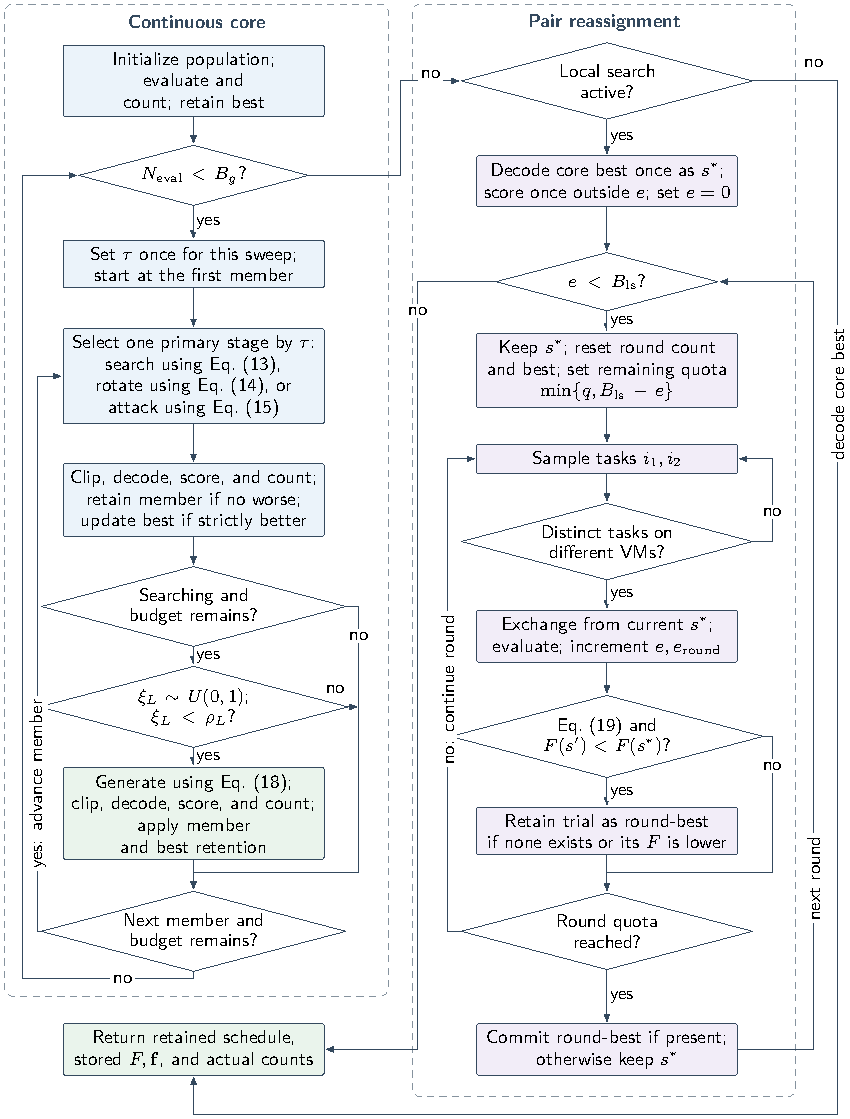
\includegraphics[width=\textwidth]{figures/publication/Fig1_LSCBO_mechanism.pdf}
\caption{Cloud LSCBO with the archived pair-sampling loop. Primary retention precedes the searching-stage L\'{e}vy trial. Local rounds use one incumbent and count every evaluated trial. Empty-neighborhood checks, attempt caps, and partial-round commits in the guarded version are specified in Algorithm~\ref{alg:lscbo}.}\label{fig:mechanism_workflow}
\end{figure}
\FloatBarrier

\subsection{Cloud Task Scheduling Using LSCBO}\label{sec:cloud_application}

\subsubsection{Schedule Representation and Initialization}\label{sec:cloud_representation}\label{sec:decoder}
A population member represents one complete candidate schedule. For $N$ tasks, the continuous dimension is $D=N$, member $h$ stores $\mathbf{X}_h=(X_{h,1},\ldots,X_{h,N})$, and its scheduling coordinates satisfy $Y_i^{(h)}=X_{h,i}$. After clipping to $[0,1]^N$, the vector $\mathbf{Y}$ is mapped to schedule $s=\mathcal{D}(\mathbf{Y})$ by
\begin{equation}\label{eq:decoder}
x_i=\min\{M-1,\lfloor MY_i\rfloor\}.
\end{equation}

The zero-based index $x_i\in\{0,\ldots,M-1\}$ corresponds to the binary assignment by $x_{i,j}=1\ \Longleftrightarrow\ x_i=j-1$, where $j$ is the one-based VM number. The interval $[r/M,(r+1)/M)$ encodes VM index $r$, with endpoint $1$ included in the last interval. The cap prevents an out-of-range index, so the decoder $\mathcal{D}$ returns a feasible assignment for every clipped vector, and every complete assignment has a representing vector. Continuous representations with problem-specific decoders are established in random-key optimization~\cite{Bean1994,GoncalvesResende2011}. Here, each coordinate independently selects a VM rather than defining a task permutation.

The Greedy-LPT reference from Section~\ref{sec:fitness} is encoded once using a dimensionless offset $\eta_x\in(0,1)$ as $Y_i=(x_i+\eta_x)/M$. This interior encoding decodes back to the reference and initializes $\mathbf{X}_1$; the other $n_{\mathrm{pop}}-1$ members are sampled independently and uniformly in $[0,1]^N$. The experimental protocol specifies the offset and other numerical settings.

The decoded objective is constant inside each interval box. A continuous displacement changes the schedule only when a coordinate crosses a decoding boundary. With fixed weights and reference denominators, deterministic finite-valued evaluation, and the reference evaluated in the initial population, every normally returned schedule satisfies $F(s_{\mathrm{out}})\leq F(s_g)$: the core retains its best evaluated schedule and local replacements strictly decrease $F$. Here $s_{\mathrm{out}}$ denotes the returned assignment. This scalar property implies neither component-wise non-regression relative to Greedy-LPT nor termination of the archived sampler. Following guidance on benchmark selection and component analysis~\cite{LaTorre2021}, we evaluate continuous search and scheduling-specific refinement separately.

\subsubsection{Candidate Evaluation}\label{sec:cloud_fitness}
Each primary or auxiliary vector is clipped, decoded by Eq.~\eqref{eq:decoder}, and scored using the analytical criteria in Section~\ref{sec4}. Fixed references $c_k$ and weights $w_k$ give the dimensionless fitness $F(\mathcal{D}(\mathbf{Y}))$ in Eq.~\eqref{eq:objective}. Comparisons and best-position retention reuse stored fitness and criteria. The continuous core compares scalar fitness; local exchanges also require Eq.~\eqref{eq:pareto_accept}.

Figure~\ref{fig:scheduling_model} connects the instance, fixed reference, continuous search, and local refinement. CloudSim Plus optionally replays the returned assignment to check executability after optimization; it never scores individual candidates.
\begin{figure}[p]
\centering
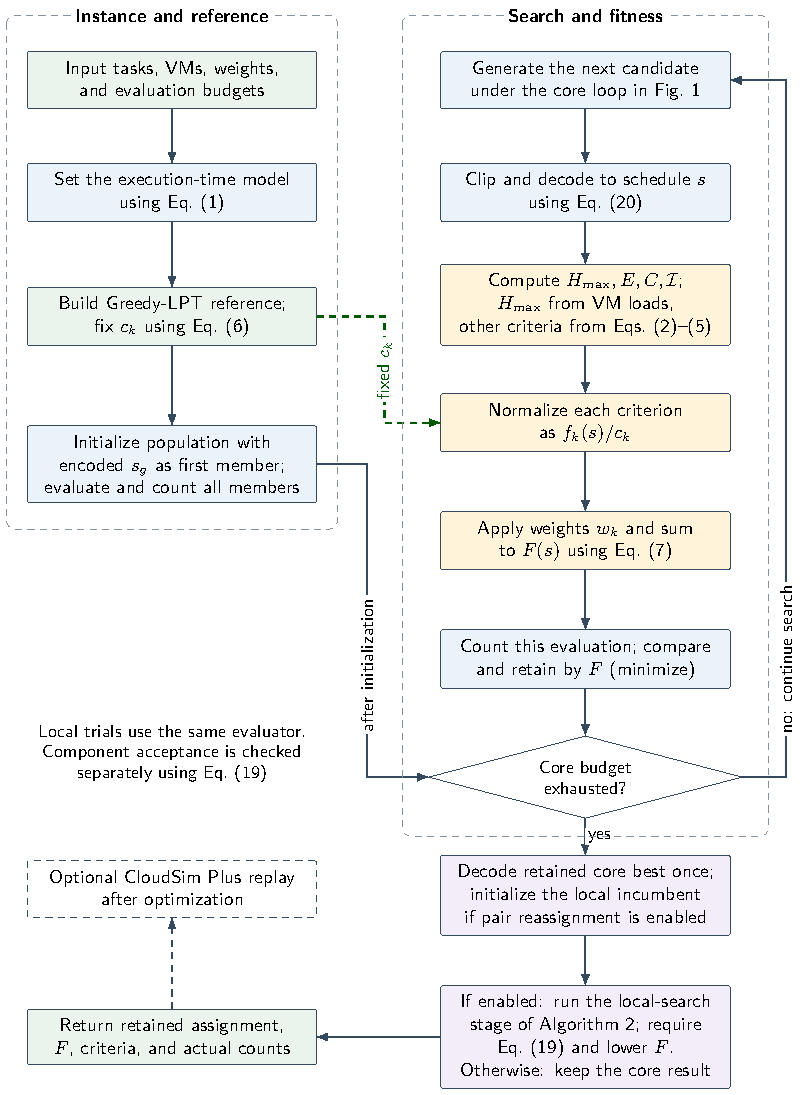
\includegraphics[width=0.99\textwidth]{figures/publication/Fig2_cloud_application.pdf}
\caption{Cloud scheduling and fitness evaluation. Initialization is scored before the core-budget check. Fixed references use Eq.~\eqref{eq:reference} and weighted fitness uses Eq.~\eqref{eq:objective}. Local trials share this evaluator and additionally require Eq.~\eqref{eq:pareto_accept} and lower $F$. Optional CloudSim replay checks the returned assignment for executability after optimization.}\label{fig:scheduling_model}
\end{figure}
\FloatBarrier

\subsubsection{Scheduling Procedure and Termination}\label{sec:cloud_procedure}
The recorded candidate allowance $B$ is divided into $B_g=\lfloor\alpha_B B\rfloor$ core evaluations and $B_{\mathrm{ls}}=B-B_g$ local evaluations, with $0<\alpha_B\leq1$ and $B_g\geq n_{\mathrm{pop}}$. When local search is disabled, the core receives the full allowance. The initialization, primary, and auxiliary evaluations all advance $N_{\mathrm{eval}}$. The L\'{e}vy trigger is drawn only after both the searching-stage and remaining-budget conditions hold.

Algorithm~\ref{alg:lscbo} integrates continuous search and pair reassignment into the complete scheduling procedure. The local count $e$ advances only after a legal candidate has been evaluated, while $e_{\mathrm{round}}$ counts such evaluations within the current round. Each round uses the remaining quota $\min\{q,B_{\mathrm{ls}}-e\}$ and samples all trials from the same incumbent. The incumbent remains unchanged if the round produces no admissible trial that strictly improves its scalar fitness. The guarded attempt cap covers illegal as well as legal draws, so its early-return count may be below the requested allowance.
\begin{algorithm}[p]
\caption{Cloud LSCBO with archived and recommended guarded pair reassignment}\label{alg:lscbo}
\small
\begin{algorithmic}[1]
\Statex \textbf{Input:} tasks, VMs, weights; even $n_{\mathrm{pop}}\geq2$; $D=N\geq2$; integer $B_g\geq n_{\mathrm{pop}}$, $B_{\mathrm{ls}}\geq0$, $q\geq1$
\Statex Local mode $m\in\{\text{none},\text{archived},\text{guarded}\}$, with $B_{\mathrm{ls}}=0$ if $m=\text{none}$; mechanism parameters as defined in Section~\ref{sec:enhancements}
\Statex \textbf{Output:} retained schedule $s^*$, $F(s^*)$, $\mathbf{f}(s^*)$, and actual counts $N_{\mathrm{eval}},e$
\State Construct $s_g$; fix its reference denominators using Eq.~\eqref{eq:reference}
\State Encode $s_g$ as $\mathbf{X}_1$; initialize remaining members as in Section~\ref{sec:cloud_representation}
\State $N_{\mathrm{eval}}\leftarrow0$; $e\leftarrow0$; $n_{\mathrm{att}}\leftarrow0$
\For{$h=1,\ldots,n_{\mathrm{pop}}$}
    \State Clip and decode $\mathbf{X}_h$; evaluate and store $F$ and $\mathbf{f}$; increment $N_{\mathrm{eval}}$ and update the retained best
\EndFor
\While{$N_{\mathrm{eval}}<B_g$}
    \State $\tau\leftarrow N_{\mathrm{eval}}/B_g$ for this population sweep
    \For{each member $h$ while $N_{\mathrm{eval}}<B_g$}
        \State Generate one primary candidate using the selected stage in Eqs.~\eqref{eq:lscbo_search}--\eqref{eq:lscbo_attack}
        \State Clip, decode, evaluate, and count it; greedily retain it and update the best using stored values
        \If{$\tau<\alpha_s$ and $N_{\mathrm{eval}}<B_g$}
            \State Draw $\xi_L\sim U(0,1)$
            \If{$\xi_L<\rho_L$}
                \State Generate the auxiliary candidate using Eq.~\eqref{eq:lscbo_levy}
                \State Clip, decode, evaluate, and count it; greedily retain it and update the best using stored values
            \EndIf
        \EndIf
    \EndFor
\EndWhile
\State Decode the retained best vector as $s^*$
\If{$m=\text{none}$}
    \State \Return $s^*,F(s^*),\mathbf{f}(s^*),N_{\mathrm{eval}},e$ using the stored evaluation
\EndIf
\State Reevaluate and store $F(s^*)$ and $\mathbf{f}(s^*)$ once outside $e$
\algstore{cloudprocedure}
\end{algorithmic}
\end{algorithm}

\begin{algorithm}[p]
\addtocounter{algorithm}{-1}
\caption{Cloud LSCBO with archived and recommended guarded pair reassignment (continued)}
\small
\begin{algorithmic}[1]
\algrestore{cloudprocedure}
\If{$m=\text{guarded}$}
    \State $A_{\max}\leftarrow\kappa_A B_{\mathrm{ls}}$
    \If{no legal cross-VM pair exists}
        \State \Return $s^*,F(s^*),\mathbf{f}(s^*),N_{\mathrm{eval}},e$
    \EndIf
\EndIf
\While{$e<B_{\mathrm{ls}}$ and ($m=\text{archived}$ or $n_{\mathrm{att}}<A_{\max}$)}
    \State $q_{\mathrm{rem}}\leftarrow\min\{q,B_{\mathrm{ls}}-e\}$; $e_{\mathrm{round}}\leftarrow0$; $s_{\mathrm{best}}\leftarrow\textsc{none}$
    \While{$e_{\mathrm{round}}<q_{\mathrm{rem}}$ and ($m=\text{archived}$ or $n_{\mathrm{att}}<A_{\max}$)}
        \If{$m=\text{guarded}$} \State $n_{\mathrm{att}}\leftarrow n_{\mathrm{att}}+1$ \EndIf
        \State Sample $i_1$ uniformly from the task indices
        \If{$m=\text{archived}$} \State $s'\leftarrow\operatorname{copy}(s^*)$ \EndIf
        \State Sample $i_2$ independently from the same task-index set
        \If{$i_1=i_2$ or the tasks occupy the same VM}
            \State \textbf{continue}
        \EndIf
        \If{$m=\text{guarded}$} \State $s'\leftarrow\operatorname{copy}(s^*)$ \EndIf
        \State Exchange the assignments in $s'$ and evaluate it
        \State $e\leftarrow e+1$; $e_{\mathrm{round}}\leftarrow e_{\mathrm{round}}+1$
        \If{Eq.~\eqref{eq:pareto_accept} holds relative to $s^*$ and $F(s')<F(s^*)$}
            \If{$s_{\mathrm{best}}=\textsc{none}$ or $F(s')<F(s_{\mathrm{best}})$}
                \State $s_{\mathrm{best}}\leftarrow s'$ with its stored evaluation
            \EndIf
        \EndIf
    \EndWhile
    \If{$s_{\mathrm{best}}\neq\textsc{none}$}
        \State $s^*\leftarrow s_{\mathrm{best}}$ with its stored evaluation
    \EndIf
\EndWhile
\State \Return $s^*,F(s^*),\mathbf{f}(s^*),N_{\mathrm{eval}},e$ using stored values
\end{algorithmic}
\end{algorithm}

The core returns its retained schedule using its stored evaluation. An active local module reevaluates that incumbent once outside the local candidate counter. Thus, internal scoring calls total $N_{\mathrm{eval}}$ without local search, or $N_{\mathrm{eval}}+e+1$ after local-module entry. These become $B$ and $B+1$, respectively, only when the corresponding candidate allowances are used in full. The shared reference-normalization evaluation is additional and is performed once per comparison instance and profile. The output is the best retained schedule under this procedure, together with its scalar objective, four criteria, and actual counts.

\FloatBarrier
\subsection{Computational Complexity}\label{sec:complexity}
Direct decoding costs $O(N)$, whereas analytical scoring costs $O(N+M)$ because it accumulates task processing loads and aggregates VM completion times into makespan, energy, cost, and load variation. Analytical scoring operates on the assignment vector without materializing the binary matrix, and both cost estimates exclude CloudSim replay.

The common warm start sorts tasks in $O(N\log N)$ and scans all VMs for each task's earliest projected finish in $O(NM)$. The scan follows MCT complexity~\cite{Braun2001}; sorting implements the additional ordering rule. Although shared conceptually across the comparison, this preprocessing remains necessary computation for each new workload.

Exchanging two assignment entries takes constant time, but archived pair search clones before checking whether the tasks occupy different VMs. Rejected draws therefore cost $O(N)$ without consuming an evaluation. Every evaluated legal exchange receives full $O(N+M)$ recomputation, including trials failing Eq.~\eqref{eq:pareto_accept}. Each round samples at most $q$ evaluated candidates rather than enumerating all pairs; failed sampling adds work. The released evaluator does not maintain incremental metrics.

Let $n_j$ count tasks on VM $j$. Independent uniform draws produce a legal pair with probability $\pi_{\mathrm{pair}}=1-\sum_{j=1}^{M}(n_j/N)^2$, invariant under exchanges. For the archived loop with $\pi_{\mathrm{pair}}>0$, the expected $1/\pi_{\mathrm{pair}}$ attempts per evaluated candidate give local cost $O(B_{\mathrm{ls}}[N/\pi_{\mathrm{pair}}+N+M])$; the loop may not terminate at $\pi_{\mathrm{pair}}=0$. The later guarded release checks empty neighborhoods, bounds attempts, and tests legality before cloning. Historical results remain attributed to the archived implementation.

Attacking scans a half-population for each candidate's leader. Let $T_{\mathrm{run}}$ denote total computational work. For a feasible initialization budget, the archived implementation has the following expected bound, conditional on the local-entry task counts and $\pi_{\mathrm{pair}}>0$. The expectation is over candidate-generation and pair-sampling randomness.

\begin{equation}\label{eq:complexity_archived}
\begin{aligned}
\mathbb{E}[T_{\mathrm{run}}]=O\bigl(&N\log N+NM+B_g(N+M+n_{\mathrm{pop}})\\
&+B_{\mathrm{ls}}[N/\pi_{\mathrm{pair}}+N+M]\bigr),\quad \pi_{\mathrm{pair}}>0.
\end{aligned}
\end{equation}

Its search term reduces to $O(B(N+M))$ when $n_{\mathrm{pop}}=O(N+M)$ and legal-pair probability is bounded away from zero. Peak active storage is $O(n_{\mathrm{pop}}N+N+M)$ for the population, assignment, and VM loads. No execution-time matrix is cached; this estimate excludes concurrent experiment replicas and the CloudSim engine.

Complexity describes workload scaling; evaluation allowances set stopping limits. Runtime also depends on implementation, hardware, and concurrent load~\cite{BartzBeielstein2020}. Experiments therefore report component ablation and descriptive timing alongside evaluation counts~\cite{LaTorre2021}.

With local search disabled, the local term and its condition on $\pi_{\mathrm{pair}}$ are omitted. For the guarded release, rejected attempts cost constant time and every valid candidate still requires full scoring. Its deterministic local cost is $O(N+M+A_{\max}+B_{\mathrm{ls}}(N+M))$, and the full-run bound replaces the last term of Eq.~\eqref{eq:complexity_archived} by $A_{\max}+B_{\mathrm{ls}}(N+M)$. The linear entry check is absorbed by the existing preprocessing and scoring terms. Early termination may leave part of the requested candidate budget unused; the recorded count must reflect actual evaluations, not the requested allowance.

\FloatBarrier

% =========================================================
% 4 Experimental Results
% =========================================================

\section{Experimental Results}\label{sec5}

Two experimental series evaluate the search core and its scheduling application. Series~1 uses CEC2017 to compare continuous optimization behavior, including a matched CBO--LSCBO comparison. Series~2 evaluates complete task assignments using the analytical model in Section~\ref{sec:model}, then examines the contribution and sensitivity of pair reassignment. A separate CloudSim Plus replay study checks the executability of a small set of returned schedules. Table~\ref{tab:series_boundary} summarizes the purposes, platforms, and compared methods of the two main series.

\begin{table}[ht]
\centering
\caption{Separation of the two validation series}\label{tab:series_boundary}
\begin{tabular}{p{0.18\textwidth} p{0.32\textwidth} p{0.40\textwidth}}
\toprule
\textbf{Series} & \textbf{Purpose and platform} & \textbf{Compared methods} \\
\midrule
Series~1 & Continuous global optimization on the official CEC2017 functions; no task-to-VM decoding or simulator is used. & LSCBO-core, adapted CBO, PSO, GWO, WOA, SA, adapted AOA, HLBO, and GWCA. \\
\midrule
Series~2 & Cloud task scheduling with direct assignment, a shared Greedy-LPT warm start, analytical multi-cost scoring, and CloudSim Plus replay support. & LSCBO, adapted CBO, PSO, GWO, WOA, adapted AOA, and Greedy-LPT; a separate matched study adds direct Greedy-LPT pair refinement. \\
\bottomrule
\end{tabular}
\end{table}

CEC2017 runs share benchmark functions and seed identifiers; cloud comparisons share task instances, VM instances, and scenario seeds. Table~\ref{tab:param_cec} gives the continuous-search settings, and Section~\ref{sec:cloud_protocol} specifies the cloud protocol.

\subsection{Experimental Series 1. CEC2017 Global Optimization Benchmarks}\label{sec:cec2017}

The display name \emph{LSCBO-core} denotes adapted CBO with auxiliary L\'{e}vy proposals, without scheduling decoding or pair reassignment; its archived data identifier remains \texttt{LSCBO}. Rotated and shifted CEC2017 functions provide a common numerical benchmark~\cite{Awad2016}. Performance is assessed by final errors and cross-function statistics, with convergence traces describing how the evaluation allowance is used.

\subsubsection{CEC2017 Settings}\label{sec:cec_settings}
All CEC2017 experiments use the official C/C++ evaluator and its official $D=30$ shift, rotation, and shuffle data. The search bounds $[-100,100]^D$ and the allowance of $10{,}000D$ evaluations follow the CEC2017 report~\cite{Awad2016}. We retain the evaluator\textquotesingle s function identifiers and evaluate F1 and F3--F30 (29 functions; F2 is excluded). Each algorithm--function cell is repeated for 30 paired seeds in this study, rather than the 51 runs specified in the competition report. Every run uses the full 300,000 evaluations, including initialization and auxiliary trials, without terminating early when error falls below $10^{-8}$. Recorded error is $\max\{0,f_{\mathrm{best}}-f_{\mathrm{opt}}\}$, where $f_{\mathrm{best}}$ is the best evaluated objective and $f_{\mathrm{opt}}$ is the known function optimum. Positive errors below $10^{-8}$ are retained, with no threshold-based zeroing before statistical aggregation. Population-based methods use 30 agents; SA is single-solution but receives the same evaluation budget. Series~1 initializes population methods directly in the continuous search domain. It does not use the Greedy-LPT warm start, task decoder, local pair reassignment, or $B_{\mathrm{ls}}$; the complete allowance is consumed by initialization and continuous candidates. The comparison set is LSCBO-core, its CBO base, PSO~\cite{Kennedy1995}, GWO~\cite{Mirjalili2014}, WOA~\cite{Mirjalili2016}, SA~\cite{Kirkpatrick1983}, adapted AOA~\cite{Abualigah2021}, HLBO~\cite{Dehghani2022HLBO}, and GWCA~\cite{Guan2023GWCA}. The CBO comparator uses the implemented core in Section~\ref{sec:enhancements}. In Series~1, the matched CBO--LSCBO-core comparison isolates the auxiliary L\'{e}vy proposal within this shared implementation; it does not compare LSCBO-core with an exact reproduction of the source paper's static CBO configuration.

The mechanism parameters in Section~\ref{sec:enhancements} are instantiated with $\alpha_s=\alpha_e=1/3$, $\delta_r=0.5$, $\theta_0=\pi$, and $\omega_A=0.5$. The additional trial uses $\rho_L=0.30$, $\lambda_L=0.03$, $\eta_L=0.05$, and $\beta=1.5$. The coordinate span is $\Delta=200$ for the CEC bounds. These fixed settings produced the archived data and were not obtained by a new tuning experiment.

The CEC implementation uses the denominator floor $\epsilon_{L,\mathrm{CEC}}=10^{-12}$ in the safeguarded Gaussian ratio defined in Section~\ref{sec:levy_step}. Algorithm names refer to the implementations evaluated in this study.

For SA, let $\tau_{\mathrm{SA}}=N_{\mathrm{eval}}/B$ include initialization immediately before each proposal. Starting from a uniformly sampled position, every coordinate receives independent Gaussian noise with standard deviation $\Delta[0.001+0.10(1-\tau_{\mathrm{SA}})]$, followed by clipping to the search bounds. The temperature is $T=1000(10^{-11})^{\tau_{\mathrm{SA}}}$. Let $\delta f$ be the candidate objective minus the current objective. A trial with $\delta f\leq0$ is accepted; otherwise its acceptance probability is $\exp[-\delta f/\max\{T,10^{-15}\}]$. The best evaluated solution is retained.

CEC PSO initializes coordinate velocities uniformly on $[-0.1\Delta,0.1\Delta]$, clips updated velocities to $[-0.2\Delta,0.2\Delta]$, and clips positions to the search bounds. At each population-sweep start, inertia is fixed to $w=0.9-0.5N_{\mathrm{eval}}/B$ and the guiding global best is copied. Every evaluated proposal replaces its current member; the personal best changes on non-increasing fitness. Cognitive and social terms use independent uniform draws with $c_1=c_2=2$.

The label \emph{adapted AOA} denotes the implementation recorded as \texttt{AOA} in the archived data. Its Math Optimizer Probability coefficient is $\mathrm{MOP}=1-\tau_{\mathrm{AOA}}^{1/5}$, and its Math Optimizer Accelerated function is $\mathrm{MOA}=0.2+0.8\tau_{\mathrm{AOA}}$, where $\tau_{\mathrm{AOA}}=N_{\mathrm{eval}}/B$ is fixed at each sweep's start. MOP controls the arithmetic step factor; MOA is the implemented multiplication/division branch probability. That branch uses $r<\mathrm{MOA}$ for a uniform draw $r$, with $\mu=0.499$, rather than the source convention $r>\mathrm{MOA}$ and $\mu=0.5$. These results therefore do not represent an exact reproduction of the original AOA. The CEC guiding best is fixed within each sweep. Candidates are clipped to the bounds and retained on non-increasing fitness. For HLBO, $R=0.2$ scales the local displacement relative to the current coordinate and the remaining generation fraction; it is not an absolute radius.

\begin{table}[ht]
\centering
\caption{Parameter settings for the CEC2017 experiments in Series~1}\label{tab:param_cec}
\begin{tabular}{l l l}
\toprule
\textbf{Algorithm} & \textbf{Parameter} & \textbf{Value} \\
\midrule
LSCBO-core & Population size & 30 \\
       & L\'{e}vy stability $\beta$ & 1.5 \\
       & Trigger probability $\rho_L$ & 0.30 \\
       & Step scale $\lambda_L$ & 0.03 \\
\midrule
Adapted CBO & Population size & 30 \\
    & Initial rotation angle $\theta_0$ & $\pi$ \\
    & Attack weight $\omega_A$ & 0.5 \\
\midrule
PSO & Population size & 30 \\
    & Inertia weight $w$ & $0.9 \rightarrow 0.4$ \\
    & Cognitive/social $c_1, c_2$ & 2.0, 2.0 \\
\midrule
SA & Initial temperature $T_0$ & 1,000 \\
   & Temperature schedule endpoint & $10^{-8}$ \\
\midrule
GWO & Population size & 30 \\
    & Convergence constant $a$ & $2 \rightarrow 0$ \\
\midrule
WOA & Population size & 30 \\
    & $a$, spiral $b$, branch probability & $2\!\rightarrow\!0$, 1, 0.5 \\
\midrule
Adapted AOA & Population size & 30 \\
    & Progress exponent $\alpha$ & 5 \\
    & Coordinate-scale parameter $\mu$ & 0.499 \\
    & Multiplication/division probability MOA & $0.2\!\rightarrow\!1$ \\
\midrule
HLBO & Population size & 30 \\
     & Relative local-update factor $R$ & 0.2 \\
\midrule
GWCA & Population size & 30 \\
     & $m,T,g,P,Q$ & 3, 8.3, 9.8, 9, 6 \\
\midrule
\multicolumn{3}{p{.95\textwidth}}{\footnotesize All methods use $D=30$, bounds $[-100,100]^D$, 30 paired runs, and 300,000 evaluations per run. In the GWCA row, the symbols $m$, $T$, and $g$ denote its mass, thrust, and gravity constants, while $P$ and $Q$ denote its Gamma shape and scale parameters; all five symbols are defined locally for this algorithm.} \\
\bottomrule
\end{tabular}
\end{table}

\FloatBarrier
\subsubsection{Performance and Statistical Comparison}\label{sec:cec_levy_ablation}
Table~\ref{tab:cec_external} summarizes the average ranks in this study using the official CEC2017 evaluator. LSCBO-core obtains the lowest average rank (1.690) over the 29 functions, ahead of SA (2.655) and PSO (3.345). At significance level $\alpha=0.05$, the Friedman test~\cite{Friedman1937} gives $\chi^2=160.313$ with eight degrees of freedom. The Iman--Davenport statistic~\cite{ImanDavenport1980} is $F_{\mathrm{ID}}=62.616$ with degrees of freedom $(8,224)$ and $p=6.18\times10^{-53}$.

The archived two-sided Wilcoxon signed-rank tests~\cite{Wilcoxon1945} use the 29 per-function mean errors, a normal approximation, and a continuity correction of 0.5, followed by Holm correction across the eight comparisons with LSCBO-core. Exact zero differences are omitted; equal absolute differences receive average ranks with a variance correction for ties. These eight comparisons contain neither zero differences nor tied absolute differences. The Iman--Davenport transformation and post-hoc procedures follow the presentation in Dem\v{s}ar~\cite{Demsar2006}. The 870 function--run observations are not pooled as independent comparison units. Because function error scales differ, signed ranks of the raw differences need not be invariant to separate positive rescaling of the functions; their magnitude-based interpretation is therefore conditional on these benchmark units.

After Holm correction, the archived tests distinguish LSCBO-core from adapted CBO, PSO, GWO, WOA, adapted AOA, HLBO, and GWCA ($p\leq0.0011$), but not from SA ($p=0.066$). The Nemenyi critical difference is approximately 2.23; the rank gaps to SA (0.97) and PSO (1.66) remain below it. These procedures answer different post-hoc questions. We report LSCBO-core as first by average rank, not as significantly superior to every comparator. Figure~\ref{fig:cec_ranking} visualizes the nine tested implementations.


Pair reassignment is not used on continuous benchmarks. In the implementation using the official CEC2017 evaluator, LSCBO-core and CBO share the same population size, three CBO phases, greedy replacement, and evaluation budget; the additional L\'{e}vy trial is their only algorithmic difference. LSCBO-core has a lower per-function mean error than CBO on all 29 functions. The paired cross-function Wilcoxon test remains significant after Holm correction ($p=2.16\times10^{-5}$). This matched comparison supports the limited conclusion that the additive L\'{e}vy trial improves the CBO core under the stated CEC2017 protocol. It does not establish universal superiority of the resulting optimizer.

\begin{table}[ht]
\centering
\caption{Friedman average ranks in this study using the official CEC2017 evaluator, with 29 functions, 30 runs, and 300,000 evaluations per run; lower is better}\label{tab:cec_external}
\begin{tabular}{l c}
\toprule
\textbf{Algorithm} & \textbf{Average rank} \\
\midrule
\textbf{LSCBO-core} & \textbf{1.690} \\
SA             & 2.655 \\
PSO            & 3.345 \\
HLBO           & 4.621 \\
GWCA           & 4.793 \\
Adapted CBO    & 5.034 \\
GWO            & 6.862 \\
Adapted AOA    & 7.448 \\
WOA            & 8.552 \\
\bottomrule
\end{tabular}
\end{table}

\begin{figure}[htbp]
\centering
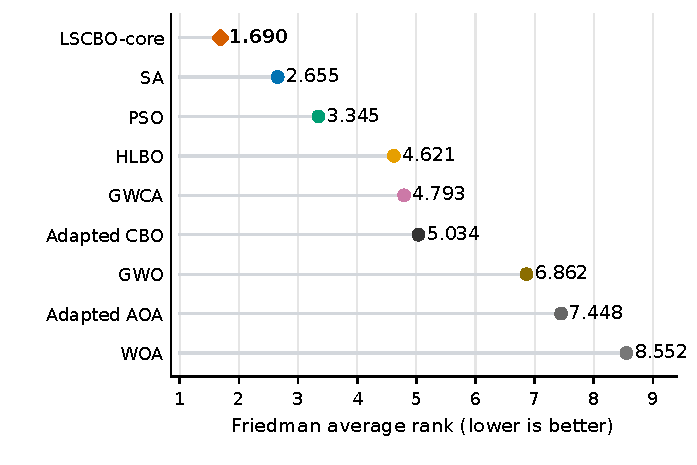
\includegraphics[width=0.90\textwidth]{figures/publication/Fig1.pdf}
\caption{Average-rank comparison in this study using the official CEC2017 evaluator. LSCBO-core obtains the best Friedman average rank (1.690) among the nine tested implementations over the 29-function, 30-run, 300,000-evaluation setting; lower rank indicates better performance.}\label{fig:cec_ranking}
\end{figure}

The comparison covers all 7,830 runs, with per-run errors, function-wise means and sample standard deviations, convergence checkpoints, and paired statistical outputs retained in the reproducibility materials.

\FloatBarrier
\subsubsection{Convergence Analysis on CEC2017}
Figure~\ref{fig:cec_convergence} reports all saved checkpoints under the complete 29-function protocol rather than selecting individual functions. LSCBO-core's mean cross-function rank improves overall, although its trajectory is non-monotonic, and reaches the final rank of 1.690 reported in Table~\ref{tab:cec_external}. Changes in relative rank can occur even when each method's best-so-far error is non-increasing. Figure~\ref{fig:cec_function_convergence} complements the aggregate rank curve with illustrative function-level traces. These trajectories are descriptive; the final paired tests remain the basis for statistical comparison.

An average rank curve emphasizes relative position within each function rather than the physical magnitude of an error reduction. A crossing of two mean rank trajectories does not imply that one method wins on every function at that checkpoint. Likewise, the selected function traces illustrate different search dynamics but are not a substitute for the full function set. For this reason, the rank trajectory, representative error curves, and final paired tests are reported as complementary summaries rather than interchangeable evidence.

\begin{figure*}[htbp]
\centering
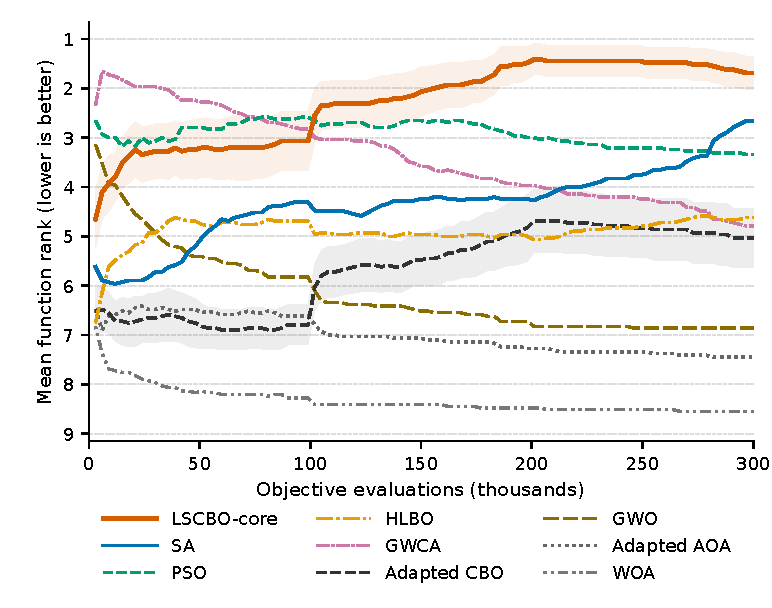
\includegraphics[width=\textwidth]{figures/publication/Fig2.pdf}
\caption{CEC2017 convergence over all 29 functions. At each checkpoint, the 30-run mean error is ranked among the nine methods within each function; curves average those ranks, with lower values indicating better performance. Shading for LSCBO-core and CBO shows descriptive pointwise normal-approximation intervals, computed as the cross-function mean rank plus or minus $1.96s_r/\sqrt{29}$, where $s_r$ is the sample standard deviation of the 29 function-specific ranks. These are neither between-run intervals nor simultaneous confidence bands.}\label{fig:cec_convergence}
\end{figure*}

\begin{figure*}[htbp]
\centering
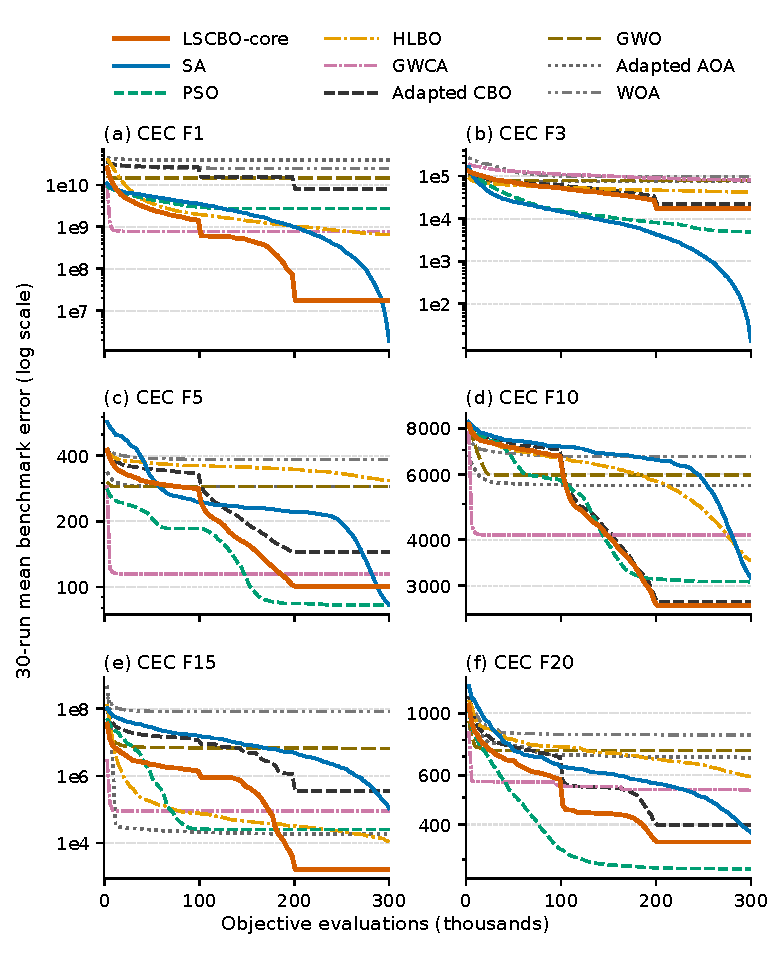
\includegraphics[width=\textwidth]{figures/publication/Fig3.pdf}
\caption{Illustrative CEC2017 convergence profiles for six benchmark functions (CEC F1, F3, F5, F10, F15, and F20). Each curve is the arithmetic mean of the best-so-far benchmark error over 30 runs, where error is the nonnegative recorded difference defined in Section~\ref{sec:cec_settings}. The mean is computed before plotting on a logarithmic axis; no additional plotting offset or clipping is applied. The CEC function identifiers are distinct from the cloud scheduling objective $F$. These six functions are not a random sample; the complete 29-function results provide the comparison evidence.}\label{fig:cec_function_convergence}
\end{figure*}

\FloatBarrier
\subsection{Experimental Series 2. Cloud Task Scheduling}\label{sec:cloudsim_exp}

\subsubsection{Experimental Settings and Protocol}\label{sec:cloud_protocol}
The formal cloud experiments use 50 heterogeneous VMs. Independent task workloads $W_i$ are sampled uniformly as integers from the inclusive range $[1000,20000]$ MI; VM processing rates are sampled uniformly as integers between the inclusive profile bounds. The default bounds are $\nu_{\mathrm{min}}=500$ and $\nu_{\mathrm{max}}=2000$ MIPS. Scenario seeds 43--72 define 30 paired instances at each task scale. The main comparison uses $N\in\{200,500,1000,2000,5000\}$; the ablation and sensitivity experiments specify their scales in the corresponding subsections. Task and VM instances use separate pseudorandom streams. Greedy-LPT orders equal-length tasks by their original indices and resolves equal projected completion times by the smallest VM index. Candidate fitness is always computed by the analytical model in Section~\ref{sec:model}.

The energy model uses $P^{\mathrm{max}}=250$ W, $\eta_P=0.6$, and $\gamma=3$, giving $P^{\mathrm{idle}}=150$ W. The conversion factor is $\kappa_t=3600$ seconds per hour. Synthetic execution-cost rates use $r_{\mathrm{min}}=0.05$ and $r_{\mathrm{max}}=0.20$ cost units per second, with $\epsilon_{\nu}=1$ MIPS. This floor is inactive for every tested capacity profile. Each profile supplies its own capacity bounds to the same price mapping. Reference floors are $\varepsilon_k^{\mathrm{ref}}=10^{-9}$ in the corresponding stored criterion units, and all reported reference values exceed them. Default weights are $w_{\mathrm{ms}}=w_{\mathrm{en}}=w_{\mathrm{cost}}=w_{\mathrm{lb}}=0.25$; local admissibility uses $\varepsilon_{\mathrm{acc}}=10^{-12}$.

LSCBO, CBO, PSO, GWO, WOA, and adapted AOA use $n_{\mathrm{pop}}=30$, a common Greedy-LPT first member, and 29 uniformly initialized members. The Greedy-LPT encoding uses the dimensionless interior offset $\eta_x=0.5$. CBO-stage and L\'{e}vy parameters retain the values reported for the continuous core, with coordinate span $\Delta=1$ and the cloud safeguard $\epsilon_{L,\mathrm{cloud}}=10^{-10}$. PSO uses $w=0.9\rightarrow0.4$ and $c_1=c_2=2$; GWO uses $a=2\rightarrow0$; WOA uses $a=2\rightarrow0$, spiral coefficient $b=1$, and branch probability 0.5; adapted AOA uses $\alpha=5$, $\mu=0.499$, and MOA increasing from 0.2 to 1.

Cloud PSO initializes each coordinate velocity as $0.1\mathcal{N}(0,1)$, clips updated velocities to $[-0.2,0.2]$ and positions to $[0,1]$, and replaces each current member with every evaluated proposal; its personal best changes only on strict improvement. Progress and inertia are fixed within each sweep, but a strictly improved global best can guide later members in that sweep. Cloud adapted AOA uses the same sweep-fixed progress schedules with arithmetic coordinate scale $0.499$; its guiding best can also update between members, and member replacement requires non-increasing fitness. The cloud optimizer uses \texttt{java.util.Random}, whereas the CEC implementation uses \texttt{std::mt19937\_64}; CEC seeds are recorded per run, while cloud optimizer seeds are derived from the scenario seed and the experiment and variant identifiers.

All population variants receive a recorded candidate allowance of $B=6000$. For local-search variants, $\alpha_B=0.10$ assigns $B_g=600$ evaluations to the core and $B_{\mathrm{ls}}=5400$ to refinement, with a per-round quota $q=400$. Population variants without local search use all 6,000 evaluations in the core. As defined in Section~\ref{sec:cloud_procedure}, local entry adds one incumbent reevaluation, giving 6,001 optimizer-internal scoring calls for the full-budget local variants and 6,000 for the others. Greedy-LPT requires one scoring call and has no core/local budget split. The candidate allowance excludes the local-entry reevaluation and the shared reference evaluation; actual scoring calls are reported separately.

Because each local round commits at most one replacement, the archived allocation permits at most $\lceil5400/400\rceil=14$ accepted exchanges. The local phase can therefore touch at most 28 distinct tasks, and fewer if tasks recur. These are procedural upper bounds, not observed acceptance counts or bounds on changes made earlier by the continuous core. The candidate allowance measures evaluated trials rather than successful schedule updates.

The analytical dataset contains 5,310 records: 1,050 main-comparison, 1,200 ablation, 2,250 weight-sensitivity, and 810 VM-heterogeneity records. Shared scenario seeds also share VM configurations across scales. Uncertainty summaries therefore resample complete seed clusters, retaining the scales within each selected cluster. The 95\% percentile intervals use 50,000 bootstrap samples with PCG64 seed 20260912. The formal results use the archived local loop in Algorithm~\ref{alg:lscbo}; the subsequent guarded implementation sets $\kappa_A=100$.

Table~\ref{tab:configuration_map} summarizes the archived configurations and their evaluation accounting.

\begin{table}[htbp]\centering\scriptsize
\caption{Archived optimizer configurations and internal scoring calls; shared reference normalization is additional}\label{tab:configuration_map}
\setlength{\tabcolsep}{2pt}
\begin{tabular}{p{.31\textwidth}p{.07\textwidth}p{.07\textwidth}p{.20\textwidth}p{.15\textwidth}p{.09\textwidth}}
\toprule Experiment / variant & Core & L\'{e}vy & Local move & $B_g/B_{\mathrm{ls}}$ & Calls \\
\midrule
E4 / LSCBO & on & on & pair-safe & 600 / 5400 & 6001 \\
E4 / CBO & on & off & none & 6000 / 0 & 6000 \\
E2 / LSCBO\_full & on & on & pair-safe & 600 / 5400 & 6001 \\
E2 / no\_levy & on & off & pair-safe & 600 / 5400 & 6001 \\
E2 / no\_local\_search & on & on & none & 6000 / 0 & 6000 \\
E2 / cbo\_base & on & off & none & 6000 / 0 & 6000 \\
E2 / ls\_only & off & off & pair-safe & 600 / 5400 & 6001 \\
E2 / objective\_only\_pair\_ls & off & off & pair-objective & 600 / 5400 & 6001 \\
E2 / pareto\_relocate\_ls & off & off & relocation-safe & 600 / 5400 & 6001 \\
Greedy-LPT & off & off & none & -- / -- & 1 \\
\bottomrule\end{tabular}
\par\smallskip{\footnotesize E4 identifies the archived main comparison; E2 identifies the mechanism ablation. Core-off variants retain initialization and unchanged-core reevaluations; they do not remove the core's entire cost. The E2 \texttt{cbo\_base} random stream differs from E4 CBO because experiment and variant labels enter the core seed. The reported scoring counts correspond to archived runs that exhaust their candidate allowances. Greedy-LPT has no population core or local-search budget; its one scoring call is listed separately. \texttt{ls\_only} retains the 30 initialization evaluations and the 570 unchanged-core reevaluations before its 5,400 local candidates; the local-search counter $e$ still counts only the 5,400 evaluated pair trials.\par}
\end{table}

\FloatBarrier

\subsubsection{Main Comparison}
Table~\ref{tab:cloud_main_objective} reports mean objective values after all four criteria are normalized by the Greedy-LPT reference. GWO, WOA, and adapted AOA match the Greedy-LPT objective and component values in every recorded block. CBO and PSO each find a lower objective in one of 150 blocks, but their aggregate changes are below 0.002\%. LSCBO with pair reassignment reduces $F$ in all 150 blocks. The matched ablation attributes this consistent difference to pair reassignment rather than to population search. Absolute component means and sample standard deviations are reported in Table~\ref{tab:main_scale_dispersion}. The separate direct-refinement comparison in Section~\ref{sec:direct_pair} reproduces the full scheduler's final assignments at the same local allowance and improves mean $F$ when its entire scoring allowance is assigned to pair search. Its results are displayed alongside the historical comparison with their separate provenance; they do not demonstrate an additional cloud benefit from retaining the continuous core.

\begin{table*}[ht]
\centering
\caption{Mean normalized scalar objective $F$ over 30 paired seeds (lower is better). Direct-refinement rows come from the separate matched runs in Section~\ref{sec:direct_pair}; their labels give the local-trial allowances.}\label{tab:cloud_main_objective}
\resizebox{\textwidth}{!}{%
\begin{tabular}{l c c c c c}
\toprule
\textbf{Method} & $N=200$ & $N=500$ & $N=1000$ & $N=2000$ & $N=5000$ \\
\midrule
LSCBO + Pareto-safe pair search & 0.982632 & 0.982617 & 0.983700 & 0.983444 & 0.985240 \\
Adapted CBO & 1.000000 & 0.999937 & 1.000000 & 1.000000 & 1.000000 \\
PSO & 0.999929 & 1.000000 & 1.000000 & 1.000000 & 1.000000 \\
GWO / WOA / adapted AOA / Greedy-LPT & 1.000000 & 1.000000 & 1.000000 & 1.000000 & 1.000000 \\
\midrule
Direct Greedy-LPT + pair, 5400 & 0.982632 & 0.982617 & 0.983700 & 0.983444 & 0.985240 \\
Direct Greedy-LPT + pair, 6000 & 0.981322 & 0.981268 & 0.982799 & 0.982076 & 0.983951 \\
\bottomrule
\end{tabular}
}
\end{table*}

\begin{table*}[ht]
\centering
\caption{Relative reductions of LSCBO over Greedy-LPT. Component reductions use scale-wise means; reductions in $F$ are means of paired instance-wise reductions. Parentheses give paired wins out of 30 seeds; all remaining cases are ties, with no component losses.}\label{tab:main_improvement}
\resizebox{\textwidth}{!}{%
\begin{tabular}{l c c c c c}
\toprule
\textbf{Scale} & \textbf{Makespan} & \textbf{Energy} & \textbf{Cost} & $\mathcal{I}$ & \textbf{Objective $F$} \\
\midrule
$N=200$  & 0.0124\% (8)  & 0.0694\% (30) & 0.0250\% (30) & 6.8139\% (30) & 1.7368\% (30) \\
$N=500$  & 0.0009\% (5)  & 0.0186\% (30) & 0.0058\% (30) & 6.6074\% (30) & 1.7383\% (30) \\
$N=1000$ & 0.0005\% (4)  & 0.0083\% (30) & 0.0028\% (30) & 6.2843\% (30) & 1.6300\% (30) \\
$N=2000$ & 0.0004\% (7)  & 0.0039\% (30) & 0.0013\% (30) & 6.4391\% (30) & 1.6556\% (30) \\
$N=5000$ & 0.0002\% (10) & 0.0014\% (30) & 0.0005\% (30) & 5.6472\% (30) & 1.4760\% (30) \\
\bottomrule
\end{tabular}
}
\end{table*}

Table~\ref{tab:main_improvement} shows nonnegative mean changes and no component losses at the recorded precision. Figure~\ref{fig:cloud_small_scale_costs}(a) presents final $F$ for the complete comparison, including the nearly overlapping CBO and PSO curves. Panel~(b) shows per-instance $100[F(s_g)-F(s)]$ reductions as dots and decomposes their mean into the weighted terms in Eq.~\eqref{eq:objective}. Each contribution is $100w_k[f_k(s_g)-f_k(s)]/c_k$ percentage points and is averaged over seeds after instance normalization. The numerical strip retains the small nonzero contributions of makespan, energy, and cost. Most of the scalar reduction comes from load imbalance. The improvement remains modest and is smallest at the largest scale, although it is not monotonic. Figure~\ref{fig:cloud_large_scale_costs} complements this comparison with component means in their original units. The recorded GWO, WOA, adapted AOA, and Greedy-LPT profiles coincide and are grouped.

\begin{figure*}[htbp]
\centering
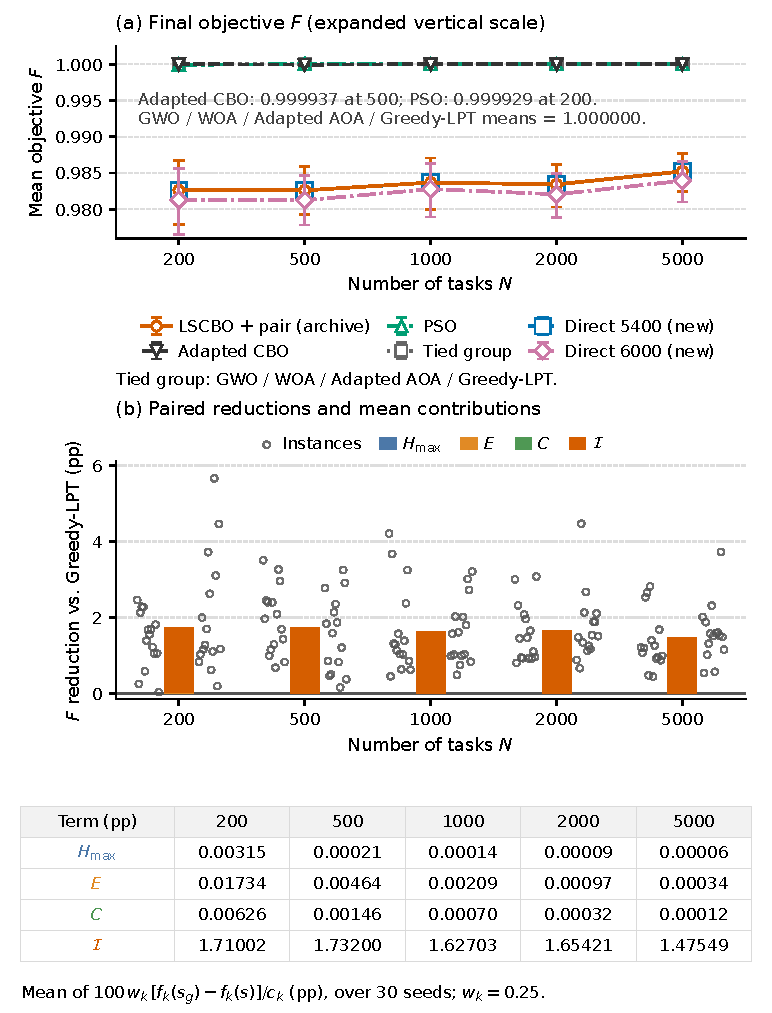
\includegraphics[width=0.995\textwidth]{figures/publication/Fig6.pdf}
\caption{Historical cloud comparison with separate direct-refinement runs. (a) Mean $F$ with pointwise 95\% seed-cluster intervals (30 outcomes per scale). Direct labels give local trials; total scoring calls are 5,402/6,002. Direct 5400 overlaps full LSCBO at plotted precision. (b) Historical full LSCBO only: paired reductions and mean contributions from Eq.~\eqref{eq:objective}. Values are percentage points of reference-normalized $F$; horizontal dot offsets distinguish seeds.}\label{fig:cloud_small_scale_costs}
\end{figure*}

\begin{figure*}[htbp]
\centering
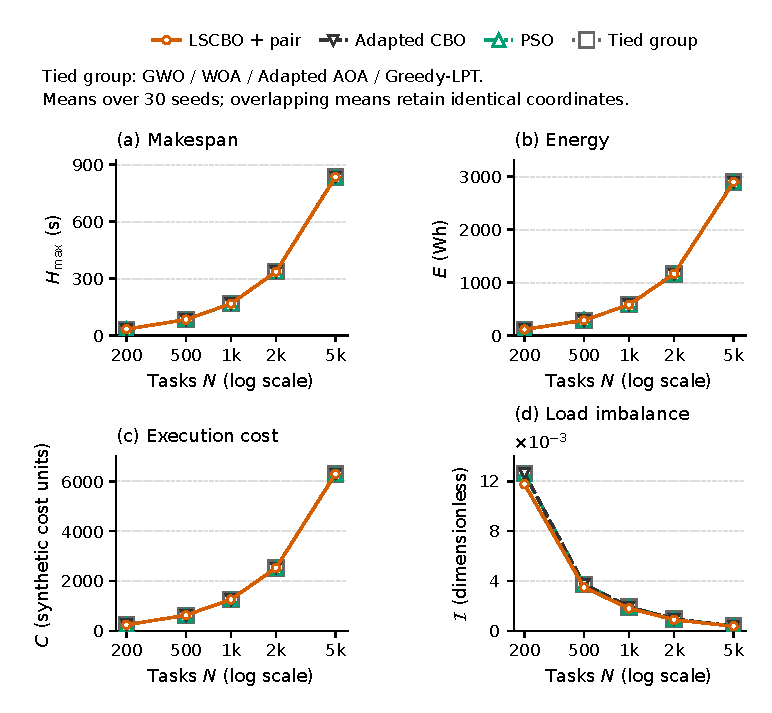
\includegraphics[width=\textwidth]{figures/publication/Fig7.pdf}
\caption{Cloud component means over 30 paired seeds at all five main-comparison scales. Panels show makespan $H_{\mathrm{max}}$ in seconds, energy $E$ in Wh, cost $C$ in synthetic cost units, and dimensionless $\mathcal{I}$ at $N\in\{200,500,1000,2000,5000\}$. Profiles for the tied GWO/WOA/adapted AOA/Greedy-LPT group are combined in each panel. The task-count axis is logarithmic ($1\mathrm{k}=1000$ tasks); all methods share the same coordinates, so coincident profiles overlap without horizontal offsets. Table~\ref{tab:main_improvement} reports paired improvement magnitudes; Table~\ref{tab:main_scale_dispersion} reports absolute sample standard deviations.}\label{fig:cloud_large_scale_costs}
\end{figure*}

\FloatBarrier

Because VM configurations are shared across task scales within each seed, the primary uncertainty analysis resamples the 30 complete seed clusters rather than treating the 150 task-count/seed blocks as independent. Using the bootstrap specified in Section~\ref{sec:cloud_protocol}, the mean paired objective reduction over Greedy-LPT is 1.6473\%, with a 95\% percentile interval of 1.4652\%--1.8351\%; the median paired reduction is 1.4584\%. This interval summarizes uncertainty for the stated synthetic-instance design and fixed task scales, not a population-wide or simulator-level guarantee.

For the historical main-comparison component counts, lower, equal, and higher values are determined by strict comparison of the CSV values stored to eight decimal places in seconds, Wh, synthetic cost units, and dimensionless imbalance. These descriptive comparisons are separate from the local acceptance tolerance. Treating component differences within $10^{-12}\max\{a_k,|f_k(s_g)|\}$ as ties leaves the counts unchanged. The $10^{-8}$ absolute tie threshold used for $F$ in the weight and capacity-profile tables is stated separately.

The paired outcomes remain useful descriptions: LSCBO records 149 objective wins and one loss against CBO, and 150 wins against each other comparator. The median objective difference from Greedy-LPT is $-0.0146$ on the reference-normalized scale. Historical block-level Friedman and Wilcoxon--Holm outputs did not account for shared-seed dependence; they are not used here as inferential evidence. For physical components, the ratio of pooled means differs from the mean of instance-wise relative improvements. The four component columns in Table~\ref{tab:main_improvement} use scale-wise ratios of means.

\begingroup
\small
\setlength{\tabcolsep}{3pt}
\renewcommand{\arraystretch}{1.10}
\begin{table}[!htbp]
\centering
\caption{Absolute analytical outcomes by task scale, reported as mean and sample standard deviation over 30 paired seeds}\label{tab:main_scale_dispersion}
\begin{tabular}{@{}p{.075\textwidth}p{.19\textwidth}p{.31\textwidth}p{.31\textwidth}@{}}
\toprule
Tasks & Metric & Greedy-LPT & LSCBO + pair search \\
\midrule

200 & Makespan (s) & 33.8687 $\pm$ 2.1541 & 33.8645 $\pm$ 2.1547 \\
200 & Energy (Wh) & 115.1420 $\pm$ 7.3617 & 115.0621 $\pm$ 7.3569 \\
200 & Cost (units) & 250.8435 $\pm$ 11.2174 & 250.7809 $\pm$ 11.2194 \\
200 & $\mathcal{I}$ & 0.01261807 $\pm$ 0.00400195 & 0.01175829 $\pm$ 0.00384325 \\
200 & Objective $F$ & 1.000000 $\pm$ 0.000000 & 0.982632 $\pm$ 0.012426 \\
500 & Makespan (s) & 84.4481 $\pm$ 3.6317 & 84.4474 $\pm$ 3.6315 \\
500 & Energy (Wh) & 291.6646 $\pm$ 12.5040 & 291.6104 $\pm$ 12.5008 \\
500 & Cost (units) & 633.7846 $\pm$ 14.4389 & 633.7476 $\pm$ 14.4403 \\
500 & $\mathcal{I}$ & 0.00374550 $\pm$ 0.00082352 & 0.00349802 $\pm$ 0.00082567 \\
500 & Objective $F$ & 1.000000 $\pm$ 0.000000 & 0.982617 $\pm$ 0.009536 \\
1000 & Makespan (s) & 168.0676 $\pm$ 7.8324 & 168.0667 $\pm$ 7.8333 \\
1000 & Energy (Wh) & 581.9240 $\pm$ 27.1202 & 581.8754 $\pm$ 27.1210 \\
1000 & Cost (units) & 1263.7005 $\pm$ 29.9877 & 1263.6649 $\pm$ 29.9897 \\
1000 & $\mathcal{I}$ & 0.00193656 $\pm$ 0.00026165 & 0.00181486 $\pm$ 0.00028253 \\
1000 & Objective $F$ & 1.000000 $\pm$ 0.000000 & 0.983700 $\pm$ 0.010073 \\
2000 & Makespan (s) & 335.9017 $\pm$ 14.7032 & 335.9004 $\pm$ 14.7033 \\
2000 & Energy (Wh) & 1164.5837 $\pm$ 50.9744 & 1164.5387 $\pm$ 50.9746 \\
2000 & Cost (units) & 2528.1930 $\pm$ 41.8799 & 2528.1610 $\pm$ 41.8825 \\
2000 & $\mathcal{I}$ & 0.00096721 $\pm$ 0.00011345 & 0.00090493 $\pm$ 0.00012407 \\
2000 & Objective $F$ & 1.000000 $\pm$ 0.000000 & 0.983444 $\pm$ 0.008343 \\
5000 & Makespan (s) & 835.4094 $\pm$ 38.4683 & 835.4074 $\pm$ 38.4680 \\
5000 & Energy (Wh) & 2898.9408 $\pm$ 133.5013 & 2898.9013 $\pm$ 133.4972 \\
5000 & Cost (units) & 6291.5506 $\pm$ 115.7708 & 6291.5192 $\pm$ 115.7681 \\
5000 & $\mathcal{I}$ & 0.00040303 $\pm$ 0.00005477 & 0.00038027 $\pm$ 0.00005991 \\
5000 & Objective $F$ & 1.000000 $\pm$ 0.000000 & 0.985240 $\pm$ 0.007489 \\
\bottomrule
\multicolumn{4}{@{}p{.97\textwidth}@{}}{\footnotesize Entries are mean $\pm$ sample standard deviation (30 seeds, divisor 29). All five task scales, four component criteria, and the scalar objective $F$ are retained. $\mathcal{I}$ and $F$ are dimensionless; cost uses the synthetic model units. Marginal dispersion across scenarios is not a confidence interval for a paired difference.}\\
\end{tabular}
\end{table}
\endgroup

Table~\ref{tab:main_scale_dispersion} exposes the absolute values and between-seed dispersion hidden by reference normalization. Mean makespan grows from 33.8687 to 835.4094 s for Greedy-LPT and from 33.8645 to 835.4074 s for LSCBO across the five scales. Energy and execution cost show the same scale dependence. Their small separations are consistent with the component improvements already reported; the raw values do not support a large reduction in execution time or resource expenditure.

Load imbalance decreases with task scale for both schedulers, while the normalized objective retains sensitivity to its relative improvement within each instance. Greedy-LPT has zero objective standard deviation because it supplies its own normalization reference, not because its physical outcomes are invariant. The displayed standard deviations describe the 30 sampled scenarios at each scale. Since methods share each scenario, uncertainty about their difference should be assessed from the paired differences and the seed-cluster analysis, rather than from overlap between these marginal summaries.

\FloatBarrier

\subsubsection{Mechanism Ablation}\label{sec:phase_ablation}
Component analysis helps distinguish the contribution of an added operator from that of the remaining algorithm~\cite{LaTorre2021}. We therefore compare variants that separate continuous updates from Pareto-safe local search. The resulting evidence concerns these components under the stated evaluation allocations.

The ablation uses the five main-comparison scales, $N\in\{200,500,1000,2000,5000\}$, with 30 paired seeds per scale. Table~\ref{tab:phase_ablation} summarizes the resulting 150 blocks per variant. LSCBO, no-L\'{e}vy CBO with local search, and the core-disabled variant have identical recorded objective and component values in all 150 blocks. The archived CSV does not store assignments, so metric equality is not treated as proof of schedule identity. The core-disabled variant tests the effect of disabling core updates, not the runtime of a fully removed core. Without local search, the recorded objective and component values match those of the reference. The tested single-task Pareto-safe relocation also yields no improvement. This result supports the effectiveness of the pair neighborhood under the sampled search procedure and evaluation budget, but does not establish its necessity. Objective-only pair search obtains a lower scalar value but slightly worsens mean energy and cost; Pareto-safe acceptance deliberately rejects such trade-offs.

Pairing refers to shared task and VM instances, not identical optimizer random streams across experiment families. The core seed is derived from the scenario seed together with the experiment and variant labels. Thus, the ablation entry labeled CBO uses the separately generated E2 \texttt{cbo\_base} runs rather than the E4 main-comparison CBO records. The local pair stream is constructed independently of the host label. This distinction explains why main-comparison CBO has a small improvement in one block while the ablation CBO row is tied throughout. Table~\ref{tab:configuration_map} specifies these configurations and their scoring counts.

\begin{table*}[ht]
\centering
\caption{Cloud mechanism ablation, averaged over 150 paired blocks. Cost uses synthetic model units; $\mathcal{I}$ and $F$ are dimensionless.}\label{tab:phase_ablation}
\resizebox{\textwidth}{!}{%
\begin{tabular}{l c c c c c}
\toprule
\textbf{Variant} & $H_{\mathrm{max}}$ (s) & $E$ (Wh) & $C$ (units) & $\mathcal{I}$ & $F$ \\
\midrule
Objective-only pair search & 291.5198 & 1010.6213 & 2193.7017 & 0.002337 & 0.899351 \\
\textbf{Pareto-safe pair search (LSCBO)} & \textbf{291.5373} & \textbf{1010.3976} & \textbf{2193.5747} & \textbf{0.003671} & \textbf{0.983527} \\
No L\'{e}vy / core-disabled pair search & 291.5373 & 1010.3976 & 2193.5747 & 0.003671 & 0.983527 \\
No local search / CBO / Greedy-LPT & 291.5391 & 1010.4510 & 2193.6144 & 0.003934 & 1.000000 \\
Pareto-safe single relocation & 291.5391 & 1010.4510 & 2193.6144 & 0.003934 & 1.000000 \\
\bottomrule
\end{tabular}
}
\end{table*}

\FloatBarrier
\subsubsection{Direct Greedy-LPT Refinement}\label{sec:direct_pair}
The archived core-disabled ablation retains repeated core scoring and therefore does not establish the value of keeping the complete search host. We conducted an additional analytical comparison on the same 150 task-count/seed instances, directly refining Greedy-LPT without population initialization or continuous candidates. The archived instance generator, evaluator, pair sampler, acceptance rule, and local random stream were reused. Before comparison, the archived full LSCBO configuration was rerun and reproduced all five recorded metrics in every block to the canonical CSV precision. These new runs are separate from the unchanged 5,310-row historical dataset.

The first direct variant uses the same 5,400 local trials as full LSCBO. The second uses 6,000 local trials, matching the full method's actual total of 6,002 scoring calls when both the reference evaluation and local-entry reevaluation are charged. It reallocates the 600 continuous evaluations to pair search. Table~\ref{tab:direct_pair} gives the quality, accepted exchanges, and elapsed times.

\begin{table}[htbp]
\centering\small
\caption{Additional direct-refinement comparison over 150 paired blocks. Mean objective reductions are relative to Greedy-LPT. Times are means of the within-block medians over five timed repetitions on the separate timing platform.}\label{tab:direct_pair}
\begin{tabular}{p{.32\textwidth}rrrr}
\toprule
Method & \shortstack{Actual\\calls} & \shortstack{$F$ reduction\\(\%)} & \shortstack{Mean accepted\\exchanges} & \shortstack{Time\\(ms)} \\
\midrule
Full LSCBO, archived path & 6002 & 1.6473 & 10.49 & 23.13 \\
Direct pair search, 5400 trials & 5402 & 1.6473 & 10.49 & 11.57 \\
Direct pair search, 6000 trials & 6002 & 1.7717 & 11.35 & 12.82 \\
\bottomrule
\end{tabular}
\end{table}

With 5,400 local trials, direct refinement and full LSCBO produce identical starting and final assignments in all 150 newly executed blocks. With 6,000 local trials, direct refinement has a lower $F$ than full LSCBO in 121 blocks and ties in 29, with no objective losses. Its additional mean reduction is 0.1244 percentage points, with a 95\% seed-cluster bootstrap interval of 0.0898--0.1632 points (50,000 resamples; PCG64 seed 20260924). No component losses against Greedy-LPT are recorded at the stored precision. This is not component-wise dominance over full LSCBO: the longer pair search has higher energy in seven blocks and higher cost in nine. The two variants can choose different admissible exchanges, each checked against its own current incumbent.

Timing was performed separately on an Apple M4 system with 16~GB RAM, macOS~27.0, and OpenJDK~25.0.2, using one application thread and a nanosecond timer. After the 150-block reproduction pass and two explicit warm-up cycles, five repetitions rotated method order across blocks. The timed region includes Greedy-LPT construction, reference normalization, and optimization; it excludes scenario generation, assignment hashing, and output. The full archived path retains its repeated Greedy-LPT construction, whereas direct refinement reuses the reference assignment. The measurements therefore compare implemented end-to-end costs, not an isolated causal cost of continuous updates. Background system load, processor frequency, and affinity were not fixed. The lower measured times of direct refinement apply to this experiment and are not portable speedup guarantees.

\FloatBarrier
\subsubsection{Weight Sensitivity}\label{sec:weight_sensitivity}
Weights in a scalarized objective affect how competing criteria influence the selected solution, and their interpretation requires care~\cite{MarlerArora2010}. We therefore test several preference profiles to assess dependence on the default equal-weight setting while retaining the individual component results. These profiles provide a preference-sensitivity check, not coverage of the complete Pareto front.

Five profiles are tested over $N\in\{100,300,500,800,1000\}$: equal weights and makespan-, energy-, cost-, and balance-priority profiles, with the emphasized criterion weighted 0.55 and each remaining criterion weighted 0.15. No component loss is recorded at the stored numerical precision. The mean objective reduction of LSCBO relative to Greedy-LPT is 1.4389\%, 0.8564\%, 0.8279\%, 0.8461\%, and 3.1607\%, respectively. It improves 148--149 of 150 blocks per profile, with the remaining blocks tied. The larger value under balance priority is consistent with the observation that pair reassignment primarily changes load imbalance. Table~\ref{tab:weight_scale_details} reports objective dispersion and paired reductions separately for each workload scale.

Changing weights changes the acceptance ranking of admissible candidates even when the component guard is retained. The resulting profiles therefore test the interaction between a declared preference and the sampled neighborhood, not the identification of a universally best preference. The detailed results below retain each workload scale so that an aggregate gain is not mistaken for a scale-independent effect. Interpretation remains conditional on the chosen weighting and normalization~\cite{MarlerArora2010}. The fixed candidate budget is part of our comparison protocol.

\begingroup
\small
\setlength{\tabcolsep}{3pt}
\renewcommand{\arraystretch}{1.10}
\begin{table}[!htbp]
\centering
\caption{Weight sensitivity at every tested task scale with LSCBO objective $F$ dispersion and paired reductions over Greedy-LPT}\label{tab:weight_scale_details}
\begin{tabular}{@{}p{.12\textwidth}p{.06\textwidth}p{.285\textwidth}p{.11\textwidth}p{.13\textwidth}p{.14\textwidth}@{}}
\toprule
Priority & Tasks & Mean $F$ $\pm$ SD & \shortstack[l]{$F$\\reduction\\(\%)} & \shortstack[l]{$\mathcal{I}$\\reduction\\(\%)} & W/T/L \\
\midrule

Equal & 100 & 0.994678 $\pm$ 0.006330 & 0.5322 & 1.8812 & 28/2/0 \\
Equal & 300 & 0.985984 $\pm$ 0.012856 & 1.4016 & 5.5581 & 30/0/0 \\
Equal & 500 & 0.982617 $\pm$ 0.009536 & 1.7383 & 6.9280 & 30/0/0 \\
Equal & 800 & 0.981074 $\pm$ 0.009821 & 1.8926 & 7.5552 & 30/0/0 \\
Equal & 1000 & 0.983700 $\pm$ 0.010073 & 1.6300 & 6.5081 & 30/0/0 \\
Makespan & 100 & 0.996608 $\pm$ 0.004005 & 0.3392 & 1.8890 & 29/1/0 \\
Makespan & 300 & 0.991108 $\pm$ 0.008810 & 0.8892 & 5.8787 & 30/0/0 \\
Makespan & 500 & 0.989373 $\pm$ 0.005378 & 1.0627 & 7.0575 & 30/0/0 \\
Makespan & 800 & 0.989671 $\pm$ 0.005208 & 1.0329 & 6.8703 & 30/0/0 \\
Makespan & 1000 & 0.990421 $\pm$ 0.004240 & 0.9579 & 6.3698 & 30/0/0 \\
Energy & 100 & 0.996227 $\pm$ 0.003912 & 0.3773 & 2.0445 & 28/2/0 \\
Energy & 300 & 0.992460 $\pm$ 0.006029 & 0.7540 & 4.8965 & 30/0/0 \\
Energy & 500 & 0.989600 $\pm$ 0.005239 & 1.0400 & 6.8681 & 30/0/0 \\
Energy & 800 & 0.990054 $\pm$ 0.004280 & 0.9946 & 6.5869 & 30/0/0 \\
Energy & 1000 & 0.990265 $\pm$ 0.005123 & 0.9735 & 6.4518 & 30/0/0 \\
Cost & 100 & 0.996418 $\pm$ 0.003947 & 0.3582 & 2.0351 & 28/2/0 \\
Cost & 300 & 0.991626 $\pm$ 0.006509 & 0.8374 & 5.5130 & 30/0/0 \\
Cost & 500 & 0.990206 $\pm$ 0.004952 & 0.9794 & 6.4898 & 30/0/0 \\
Cost & 800 & 0.989198 $\pm$ 0.006045 & 1.0802 & 7.1766 & 30/0/0 \\
Cost & 1000 & 0.990247 $\pm$ 0.005630 & 0.9753 & 6.4827 & 30/0/0 \\
Balance & 100 & 0.988316 $\pm$ 0.013521 & 1.1684 & 2.0553 & 29/1/0 \\
Balance & 300 & 0.968953 $\pm$ 0.029727 & 3.1047 & 5.6333 & 30/0/0 \\
Balance & 500 & 0.959437 $\pm$ 0.020384 & 4.0563 & 7.3680 & 30/0/0 \\
Balance & 800 & 0.960283 $\pm$ 0.018853 & 3.9717 & 7.2174 & 30/0/0 \\
Balance & 1000 & 0.964974 $\pm$ 0.018062 & 3.5026 & 6.3649 & 30/0/0 \\
\bottomrule
\multicolumn{6}{@{}p{.97\textwidth}@{}}{\footnotesize Each row summarizes outcomes across 30 paired scenario seeds. Equal weights are (0.25,0.25,0.25,0.25); a priority weight is 0.55 and the others are 0.15. The $F$ and $\mathcal{I}$ reductions are means of per-instance percentage reductions, not ratios of pooled means. Greedy-LPT has objective 1.000000 $\pm$ 0.000000 in every row. W/T/L compares $F$ using an absolute statistical tie tolerance of $10^{-8}$ on $F$ differences; SD is the sample standard deviation.}\\
\end{tabular}
\end{table}
\endgroup

Table~\ref{tab:weight_scale_details} localizes the few ties in the weight experiment, all of which occur at 100 tasks. At this scale, equal, energy-priority, and cost-priority weights yield 28 wins and two ties, while makespan and balance priority yield 29 wins and one tie. Every profile improves all 30 blocks at each of the four larger scales. Pooling scales therefore conceals a difference between the smallest workload and the remaining tested workloads.

Balance priority produces the largest mean objective reduction at every tested scale, ranging from 1.1684\% to 4.0563\%. This pattern should be interpreted alongside the load imbalance column and the change in scalarization weights because a larger reduction in a differently weighted objective is not directly a larger physical benefit. The scale-specific standard deviations also show substantial instance variation, particularly for balance priority. The complete set of cells supports sensitivity to preference and workload size without implying that any one weight vector is generally optimal.

\FloatBarrier

\subsubsection{VM Heterogeneity}\label{sec:vm_heterogeneity}
Resource heterogeneity is varied through the configured VM-speed range, an experimental dimension of static mapping~\cite{Braun2001}. The processing rate $\nu_j$ is sampled uniformly from the inclusive integer ranges $[1333,2000]$, $[400,2000]$, and $[100,2000]$ MIPS, labeled approximately 1.5:1, 5:1, and 20:1; the first label abbreviates $2000/1333$. Each profile uses $N\in\{500,1000,2000\}$ and 30 paired seeds with equal weights. The separable execution-time model and capacity-dependent price mapping remain as defined in Section~\ref{sec:model}.

Across the 90 blocks per profile, mean LSCBO objectives are 0.997258, 0.985625, and 0.994473, respectively, against the Greedy-LPT reference of 1.000000. The near-homogeneous profile has 38 wins and 52 ties; both other profiles improve every block. Table~\ref{tab:heterogeneity_scale_details} resolves these results by task scale, and Figure~\ref{fig:ablation_robustness} summarizes the profile-wise reductions.

\begingroup
\small
\setlength{\tabcolsep}{3pt}
\renewcommand{\arraystretch}{1.10}
\begin{table}[!htbp]
\centering
\caption{VM-capacity profiles by task scale with LSCBO objective $F$ and paired reductions over Greedy-LPT}\label{tab:heterogeneity_scale_details}
\begin{tabular}{@{}p{.12\textwidth}p{.06\textwidth}p{.285\textwidth}p{.11\textwidth}p{.13\textwidth}p{.14\textwidth}@{}}
\toprule
Capacity ratio & Tasks & Mean $F$ $\pm$ SD & \shortstack[l]{$F$\\reduction\\(\%)} & \shortstack[l]{$\mathcal{I}$\\reduction\\(\%)} & W/T/L \\
\midrule

1.5:1 & 500 & 0.993851 $\pm$ 0.005751 & 0.6149 & 2.4595 & 22/8/0 \\
1.5:1 & 1000 & 0.999034 $\pm$ 0.002241 & 0.0966 & 0.3865 & 12/18/0 \\
1.5:1 & 2000 & 0.998889 $\pm$ 0.003331 & 0.1111 & 0.4445 & 4/26/0 \\
5:1 & 500 & 0.985343 $\pm$ 0.009439 & 1.4657 & 5.8316 & 30/0/0 \\
5:1 & 1000 & 0.984386 $\pm$ 0.006551 & 1.5614 & 6.2336 & 30/0/0 \\
5:1 & 2000 & 0.987147 $\pm$ 0.006688 & 1.2853 & 5.1350 & 30/0/0 \\
20:1 & 500 & 0.993056 $\pm$ 0.006740 & 0.6944 & 2.7348 & 30/0/0 \\
20:1 & 1000 & 0.995010 $\pm$ 0.003083 & 0.4990 & 1.9765 & 30/0/0 \\
20:1 & 2000 & 0.995353 $\pm$ 0.004762 & 0.4647 & 1.8502 & 30/0/0 \\
\bottomrule
\multicolumn{6}{@{}p{.97\textwidth}@{}}{\footnotesize The capacity ratio is $\nu_{\mathrm{max}}/\nu_{\mathrm{min}}$ for the configured processing-rate bounds. Each cell contains 30 seeds and 50 VMs, with equal objective weights. The $F$ and $\mathcal{I}$ reduction columns are means of paired instance-wise percentage reductions. Greedy-LPT has objective 1.000000 $\pm$ 0.000000 in every cell. W/T/L uses an absolute statistical tie tolerance of $10^{-8}$ on $F$ differences. Each capacity profile also changes its capacity-normalized price mapping.}\\
\end{tabular}
\end{table}
\endgroup

All objective ties occur under the near-homogeneous profile, whose wins decline from 22 of 30 blocks at 500 tasks to 12 at 1,000 and four at 2,000, with mean reductions of 0.6149\%, 0.0966\%, and 0.1111\%. At every matched scale, the mean $F$ reduction is larger under the 5:1 profile than under the 20:1 profile, so a wider capacity range does not imply a larger benefit. Each profile changes both speeds and their price mapping; these observations describe resource-profile sensitivity without isolating a causal speed effect. Figure~\ref{fig:ablation_robustness} summarizes sensitivity to the tested weight and VM-capacity profiles.

\begin{figure*}[htbp]
\centering
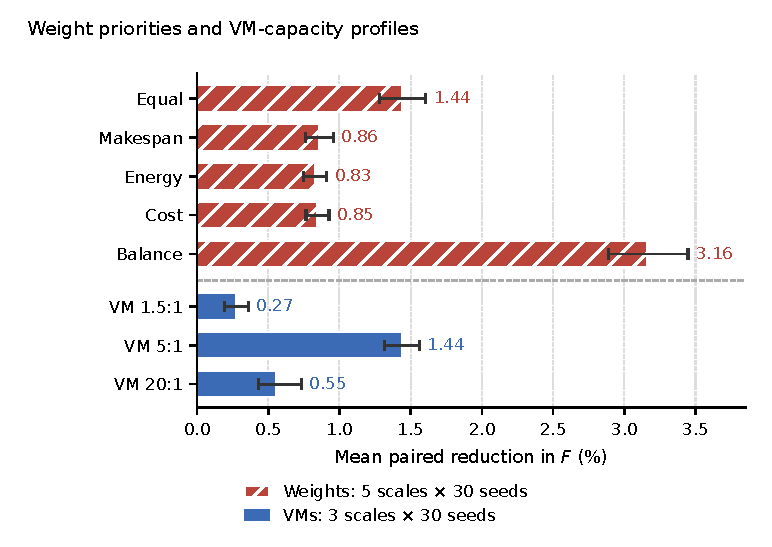
\includegraphics[width=0.99\textwidth]{figures/publication/Fig8.pdf}
\caption{Weight and VM-capacity sensitivity. Mean paired reductions in $F$ relative to Greedy-LPT across five weight profiles (five task scales each) and three VM-capacity profiles (three task scales each). Error bars show 95\% seed-cluster bootstrap intervals based on 30 seeds and 50,000 resamples using PCG64 seed 20260912; each cluster retains all tested scales.}\label{fig:ablation_robustness}
\end{figure*}

\FloatBarrier
\subsubsection{Descriptive Runtime Analysis}\label{sec:runtime_descriptive}
The elapsed-time measurements complement the evaluation counts and complexity analysis~\cite{BartzBeielstein2020}. Table~\ref{tab:runtime_descriptive} reports medians and quartiles from the analytical main comparison.

The logs were collected with 16 concurrent workers and millisecond timestamps. Timing includes optimization and Greedy-LPT construction, but excludes scenario generation and shared normalization. No JVM warm-up protocol or complete physical machine configuration is recorded. Consequently, these values describe the archived run conditions and do not establish portable speedups; a zero-millisecond entry reflects timer resolution.

\begin{table}[htbp]
\centering
\caption{Archived main-comparison runtime in milliseconds, reported as median [first quartile, third quartile] over 30 seeds. These are concurrent logs, not controlled timing benchmarks.}\label{tab:runtime_descriptive}
\begin{tabular}{l c c}
\toprule
Tasks & Greedy-LPT & LSCBO with pair search \\
\midrule
200 & 0.0 [0.0, 0.0] & 27.5 [16.25, 46.5] \\
500 & 0.0 [0.0, 0.0] & 32.5 [25.25, 47.0] \\
1000 & 0.0 [0.0, 0.0] & 45.5 [39.25, 55.0] \\
2000 & 0.0 [0.0, 1.0] & 69.0 [59.25, 78.0] \\
5000 & 1.0 [1.0, 1.75] & 173.0 [148.0, 182.5] \\
\bottomrule
\end{tabular}
\end{table}

In the separate matched ablation, mean recorded times for the full, no-L\'{e}vy, and core-disabled variants are 121.45, 102.04, and 78.27 ms, respectively, with identical recorded objective and component values. The full variant exceeds the core-disabled variant by a mean paired 43.19 ms and a median paired 36.00 ms. These concurrent logs do not establish isolated speedups, causal core overhead, or the cost of a fully simplified Greedy-LPT-plus-local-search implementation. Section~\ref{sec:direct_pair} reports the additional direct-refinement experiment on a separately documented platform; its timings must not be pooled with these historical measurements.

\FloatBarrier

\subsection{CloudSim Plus Replay Validation}\label{sec:replay_validation}
The analytical evaluator and the simulator answer different questions. The former supplies every candidate's fitness; the latter checks whether a returned assignment executes under the configured scheduling policies. The replay uses CloudSim Plus~\cite{SilvaFilho2017}, which builds on CloudSim~\cite{Calheiros2011}; version 8.0.0 is used here. Hosts have four cores, 16 GB RAM, 1 TB storage, and 10 Gbps bandwidth, with the datacenter expanding beyond the initial 10 hosts when needed. Hosts use VmSchedulerSpaceShared and VMs use CloudletSchedulerTimeShared. The archived replay entry point is \texttt{ClaimPreservingCloudSimExperiment} with \texttt{--mode smoke}. Its implementation creates one-processing-element VMs with MIPS equal to $\nu_j$ and one-processing-element cloudlets of length $W_i$ MI, using \texttt{UtilizationModelFull} for CPU demand. Both lists are submitted to the broker before simulation starts. Cloudlet submission delay and the datacenter scheduling interval retain their CloudSim Plus 8.0.0 defaults of zero; these settings do not imply execution starts at simulation time zero.

The replay set contains 12 runs of LSCBO, CBO, and Greedy-LPT on 50 or 100 tasks, 10 VMs, and seeds 43 and 44, providing four paired scenarios. These settings are smaller than the 50-VM analytical experiments and were not used to score the formal candidate searches. Table~\ref{tab:complete_smoke_replay} reports analytical and simulated makespan for every archived replay.

\begin{table}[!htbp]
\centering\small
\setlength{\tabcolsep}{3pt}
\caption{Complete CloudSim Plus smoke replay with analytical and simulated makespan for all 12 archived runs}\label{tab:complete_smoke_replay}
\begin{tabular}{@{}p{.065\textwidth}p{.065\textwidth}p{.16\textwidth}p{.17\textwidth}p{.17\textwidth}p{.13\textwidth}p{.1\textwidth}@{}}
\toprule
Tasks & Seed & Method & Analytical (s) & Replay (s) & Replay $\Delta$ vs. Greedy-LPT (s) & Finished \\
\midrule

50 & 43 & LSCBO & 35.78591 & 36.14320 & -0.04807 & 50 \\
50 & 43 & CBO & 35.78591 & 36.19127 & 0.00000 & 50 \\
50 & 43 & Greedy-LPT & 35.78591 & 36.19127 & 0.00000 & 50 \\
50 & 44 & LSCBO & 35.31143 & 35.76710 & +0.09796 & 50 \\
50 & 44 & CBO & 35.31722 & 35.66914 & 0.00000 & 50 \\
50 & 44 & Greedy-LPT & 35.31722 & 35.66914 & 0.00000 & 50 \\
100 & 43 & LSCBO & 73.54318 & 75.04496 & +0.06777 & 100 \\
100 & 43 & CBO & 73.54318 & 74.97719 & 0.00000 & 100 \\
100 & 43 & Greedy-LPT & 73.54318 & 74.97719 & 0.00000 & 100 \\
100 & 44 & LSCBO & 75.08252 & 76.34868 & -0.32669 & 100 \\
100 & 44 & CBO & 75.15959 & 76.67537 & 0.00000 & 100 \\
100 & 44 & Greedy-LPT & 75.15959 & 76.67537 & 0.00000 & 100 \\

\bottomrule
\multicolumn{7}{@{}p{.97\textwidth}@{}}{\footnotesize All requested cloudlets finish in every run, each of which uses 10 VMs. Difference is replay makespan minus Greedy-LPT replay makespan in the same task-count/seed block; negative values favor the listed method. This smoke configuration differs from the 50-VM formal analytical experiments and supplies four paired scenarios, not 12 independent comparisons.}\\
\end{tabular}
\end{table}
\FloatBarrier


Table~\ref{tab:complete_smoke_replay} reports every archived replay, including the two scenarios in which LSCBO has a higher simulated makespan than Greedy-LPT. The four paired differences are $-0.04807$, $+0.09796$, $+0.06777$, and $-0.32669$ s in table order. CBO matches Greedy-LPT in all four replays. Completion counts equal the requested task counts for every method, so the complete record supports schedule executability while preserving the unfavorable simulated outcomes.

Simulated makespan exceeds the corresponding analytical value in all 12 records, and an analytical improvement does not determine the sign of the paired replay difference. These observations separate assignment executability from the ability of the analytical objective to predict simulator-level ordering. The smoke experiment addresses the former for four small scenarios. Its task counts, VM count, and sample size do not support numerical equivalence with the main experiment or a simulator-level non-regression claim.

\FloatBarrier

\section{Discussion}\label{sec6}

\textbf{What the combined objective measures.}
Greedy-LPT is a strong baseline in the tested independent-task setting. Pair reassignment reduces the reference-normalized objective by 1.48\%--1.74\% across scales, while the relative load imbalance reduction is 5.65\%--6.81\%. Mean load imbalance changes from 0.003934 to 0.003671. Reductions in makespan, energy, and cost are below 0.01\% when computed as ratios of pooled means. Under equal weights, load imbalance contributes approximately 1.63975 percentage points of the 1.64733-point mean objective reduction, or 99.54\%. Makespan, energy, and cost contribute approximately 0.00073, 0.00508, and 0.00177 points. These contributions explain the normalized objective, rather than implying comparable physical savings across criteria. At 5,000 tasks, for example, mean $\mathcal{I}$ falls from 0.00040303 to 0.00038027, an absolute change of about $2.28\times10^{-5}$. No service-level threshold or deployment measurement is available to establish the operational value of that change. Consistent paired improvements can therefore coexist with a small operational effect.

\textbf{Why the acceptance condition matters.}
Objective-only pair search reduces the normalized objective by 10.06\% and load imbalance by 40.59\%, but worsens makespan in 30 blocks, energy in 147, and cost in 148 relative to Greedy-LPT. For a given incumbent, the component-wise condition restricts the admissible exchange set relative to scalar-only acceptance. This restriction is consistent with the smaller observed scalar benefit, but does not by itself determine how many exchanges different search paths commit. The observed absence of component losses against Greedy-LPT in the main experiment is an empirical result; the acceptance rule itself applies to the current incumbent.

\textbf{Which mechanism supplies the benefit.}
The cloud ablation gives identical recorded metrics for LSCBO, no-L\'{e}vy CBO with pair search, and the core-disabled pair-search variant. The additional direct-refinement experiment strengthens this finding: removing the population core yields identical final assignments under the same local budget, while reallocating its scoring allowance to pair search improves the mean scalar outcome. The tested cloud results therefore support pair refinement under component-wise tolerances rather than an additional benefit from the continuous CBO--L\'{e}vy host. This conclusion is conditional on the stated decoder, initialization, instance family, local random stream, and evaluation allocations. The decoder's constant-fitness regions offer a possible explanation, but the experiments do not isolate a unique cause. Nor do they establish that pair reassignment has the same effect with every other host optimizer. The CEC2017 evidence addresses a different question: the L\'{e}vy addition improves the implemented CBO on all 29 functions, although LSCBO-core is not distinguished from SA after correction. Continuous benchmark performance therefore cannot substitute for scheduling-specific evidence.

\textbf{Scope and limitations.}
The model considers offline scheduling of independent tasks and omits precedence constraints, communication delays, failures, and dynamic arrivals. Task lengths are synthetic, the formal tests retain 50 VMs, and the power and price functions are analytical approximations. The selected weights and Greedy-LPT reference define the meaning of $F$; preference sensitivity does not establish a universally best weighting or a complete Pareto front. Pair exchange preserves per-VM task counts, and finite random sampling does not establish exhaustive local optimality. The additional experiment compares two local allowances with the same round quota, not a broad budget or neighborhood-size sweep. Its timing uses one platform and does not establish online scheduling suitability.

The four paired CloudSim replays demonstrate executability but yield two makespan improvements and two regressions. They do not validate simulator-level non-regression or the full analytical dataset. Comparisons with exact small-instance optima, production traces, and learning-based schedulers are also absent. The present contribution is therefore a measured, component-controlled refinement under the stated model, with broader scheduling benefits left for further evaluation.

\section{Conclusion and Future Work}\label{sec7}

This study evaluated task-pair refinement under component-wise tolerances within a CBO--L\'{e}vy scheduling framework and as a direct refinement of Greedy-LPT. A fixed Greedy-LPT reference links the four analytical criteria to one scalar objective, while the local acceptance condition controls component-level trade-offs relative to the incumbent.

Across 150 paired cloud instances, the scheduler lowers $F$ in every block with a mean reduction of 1.65\% and no recorded component losses against Greedy-LPT. Most of this reduction comes from load imbalance. Ablation identifies pair reassignment as the effective refinement under the tested conditions. An additional experiment directly refines Greedy-LPT and obtains the same final schedules with 5,400 local trials; with the complete scoring allowance reassigned to 6,000 local trials, its mean objective reduction increases to 1.77\%. These results do not demonstrate an additional cloud benefit from retaining the continuous core. In the separate CEC2017 study, LSCBO-core ranks first among nine methods but is not significantly different from SA after correction. The small CloudSim replay study yields two makespan improvements and two regressions, limiting the observed component-wise non-regression to the tested analytical instances; it is not a general guarantee of the complete framework.

Future work should examine how the pair operator transfers to other search hosts, vary local budgets and round quotas, test precedence-constrained workflows and real traces, and use exact small-instance optima to assess solution quality. Calibrated energy and price models, service-level criteria, and broader simulator replay are needed to determine whether the analytical improvements translate into operational benefits.

\section*{Statements and Declarations}
\textbf{Funding} See Acknowledgments.

\textbf{Competing Interests} The authors declare no competing interests.

\textbf{Author Contributions} Yarui Yuan and Yubo Wang contributed to the study conception, algorithm design, implementation, experiments, analysis, and manuscript preparation, and approved the final manuscript.

\textbf{Data Availability} The original study's repository is available at \url{https://github.com/Lazywords2006/LSCBO}. The canonical evidence comprises 5,310 analytical cloud records, 12 CloudSim Plus smoke-replay records, and 7,830 per-run CEC2017 results. The additional direct-refinement analysis uses 2,250 timed records from 150 paired instances, three methods, and five repetitions; timing repetitions are not counted as additional independent quality instances. Its protocol, validation and summary results are reported in Section~\ref{sec:direct_pair}. Raw data files are separate from the article. Full CloudSim replay of the formal dataset is not included.

\textbf{Code Availability} The original experiment code is associated with the public repository at \url{https://github.com/Lazywords2006/LSCBO}. Sections~\ref{sec:enhancements} and~\ref{sec:cloud_procedure} distinguish the implemented adaptation and local-search versions. The additional study in Section~\ref{sec:direct_pair} reuses the archived scheduling and evaluation rules without modifying the canonical datasets; later instrumentation and safeguards are not attributed to the historical experiments. The CEC result manifest is labeled \texttt{official-cec2017-d30-v1}. SHA-256 prefixes \texttt{9c0a9ae26945} (CEC \texttt{classic.cpp}) and \texttt{390a349cb86c} (archived cloud implementation) identify the comparator source snapshots; they do not by themselves establish the identity of historical executables.


\textbf{AI Tool Usage} AI-assisted tools were used during manuscript preparation for language editing, consistency checking, and formatting support. All experimental design, data analysis, scientific claims, and final manuscript decisions were reviewed and verified by the authors.

\textbf{Ethics Approval} Not applicable.

\textbf{Consent to Participate} Not applicable.

\textbf{Consent for Publication} Not applicable.

\section*{Acknowledgments}
This work was supported by the Natural Science Foundation of Xiamen, China (3502Z202374058) and the Educational Research Project for Young and Middle-aged Teachers of Fujian Province (JAS23220).










% =========================================================
% References
% =========================================================

\setlength{\bibsep}{0.65em}
\begin{thebibliography}{52}
\interlinepenalty=10000

\bibitem{Armbrust2010}
Armbrust M, Fox A, Griffith R, Joseph AD, Katz R, Konwinski A, Lee G, Patterson D, Rabkin A, Stoica I, Zaharia M (2010) A view of cloud computing. Commun ACM 53(4):50--58. \url{https://doi.org/10.1145/1721654.1721672}

\bibitem{Buyya2009}
Buyya R, Yeo CS, Venugopal S, Broberg J, Brandic I (2009) Cloud computing and emerging IT platforms: vision, hype, and reality for delivering computing as the 5th utility. Future Gener Comput Syst 25(6):599--616. \url{https://doi.org/10.1016/j.future.2008.12.001}

\bibitem{Coffman1976}
Coffman EG Jr (ed) (1976) Computer and Job-Shop Scheduling Theory. Wiley, New York.

\bibitem{Braun2001}
Braun TD, Siegel HJ, Beck N, B\"{o}l\"{o}ni LL, Maheswaran M, Reuther AI, Robertson JP, Theys MD, Yao B, Hensgen D, Freund RF (2001) A comparison of eleven static heuristics for mapping a class of independent tasks onto heterogeneous distributed computing systems. J Parallel Distrib Comput 61(6):810--837. \url{https://doi.org/10.1006/jpdc.2000.1714}

\bibitem{Etminani2007}
Etminani K, Naghibzadeh M (2007) A Min-Min Max-Min selective algorithm for grid task scheduling. Proc 3rd IEEE/IFIP Int Conf Cent Asia Internet 1--7. \url{https://doi.org/10.1109/CANET.2007.4401694}

\bibitem{Kennedy1995}
Kennedy J, Eberhart R (1995) Particle swarm optimization. Proc ICNN'95-Int Conf Neural Networks 4:1942--1948. \url{https://doi.org/10.1109/ICNN.1995.488968}

\bibitem{Goldberg1989}
Goldberg DE (1989) Genetic algorithms in search, optimization, and machine learning. Addison-Wesley, Reading, MA.

\bibitem{Yang2014}
Yang XS (2014) Nature-Inspired Optimization Algorithms, 1st edn. Elsevier. ISBN 978-0-12-416743-8.

\bibitem{Mirjalili2016}
Mirjalili S, Lewis A (2016) The whale optimization algorithm. Adv Eng Softw 95:51--67. \url{https://doi.org/10.1016/j.advengsoft.2016.01.008}

\bibitem{Mirjalili2014}
Mirjalili S, Mirjalili SM, Lewis A (2014) Grey wolf optimizer. Adv Eng Softw 69:46--61. \url{https://doi.org/10.1016/j.advengsoft.2013.12.007}

\bibitem{Xue2022}
Xue J, Shen B (2023) Dung beetle optimizer: a new meta-heuristic algorithm for global optimization. J Supercomput 79:7305--7336. \url{https://doi.org/10.1007/s11227-022-04959-6}

\bibitem{Abualigah2021}
Abualigah L, Diabat A, Mirjalili S, Abd Elaziz M, Gandomi AH (2021) The arithmetic optimization algorithm. Comput Methods Appl Mech Eng 376:113609. \url{https://doi.org/10.1016/j.cma.2020.113609}

\bibitem{Khatab2025}
Khatab M, El-Gamel M, Saleh AI, El-Shenawy A, Rabie AH (2025) Coyote and Badger Optimization (CBO): a natural inspired meta-heuristic algorithm based on cooperative hunting. Commun Nonlinear Sci Numer Simul 140:108333. \url{https://doi.org/10.1016/j.cnsns.2024.108333}

\bibitem{Chintale2024}
Chintale P, Malviya RK, Merla NB, Chinna PPG, Desaboyina G, Sure TAR (2024) Levy flight osprey optimization algorithm for task scheduling in cloud computing. Proc 2024 Int Conf Intell Algorithms Comput Intell Syst (IACIS) 1--5. \url{https://doi.org/10.1109/IACIS61494.2024.10721633}

\bibitem{Sabipour2025}
Sabipour MR, Sayadnavard MH (2025) A chaotic RIME optimization algorithm based on generalized quadratic interpolation with L\'{e}vy flight for task scheduling in cloud computing. J Soft Comput Inf Technol 14(1):57--67. \url{https://doi.org/10.22034/jscit.2025.220413}

\bibitem{Zhu2025}
Zhu M, Li J, Yang X (2025) A hybrid SAO and RIME optimizer for global optimization and cloud task scheduling. Biomimetics 10(10):690. \url{https://doi.org/10.3390/biomimetics10100690}

\bibitem{Deb2002}
Deb K, Pratap A, Agarwal S, Meyarivan T (2002) A fast and elitist multiobjective genetic algorithm: NSGA-II. IEEE Trans Evol Comput 6(2):182--197. \url{https://doi.org/10.1109/4235.996017}

\bibitem{Zhang2007}
Zhang Q, Li H (2007) MOEA/D: a multiobjective evolutionary algorithm based on decomposition. IEEE Trans Evol Comput 11(6):712--731. \url{https://doi.org/10.1109/TEVC.2007.892759}

\bibitem{Mantegna1994}
Mantegna RN (1994) Fast, accurate algorithm for numerical simulation of L\'{e}vy stable stochastic processes. Phys Rev E 49(5):4677--4683. \url{https://doi.org/10.1103/PhysRevE.49.4677}

\bibitem{Kirkpatrick1983}
Kirkpatrick S, Gelatt CD Jr, Vecchi MP (1983) Optimization by simulated annealing. Science 220(4598):671--680. \url{https://doi.org/10.1126/science.220.4598.671}

\bibitem{Verma2017}
Verma A, Kaushal S (2017) A hybrid multi-objective Particle Swarm Optimization for scientific workflow scheduling. Parallel Comput 62:1--19. \url{https://doi.org/10.1016/j.parco.2017.01.002}

\bibitem{AbdelBasset2023}
Abdel-Basset M, Mohamed R, Azeem SAA, Jameel M, Abouhawwash M (2023) Kepler optimization algorithm: a new metaheuristic algorithm inspired by Kepler's laws of planetary motion. Knowl-Based Syst 268:110454. \url{https://doi.org/10.1016/j.knosys.2023.110454}

\bibitem{Hashim2022}
Hashim FA, Hussien AG (2022) Snake optimizer: a novel meta-heuristic optimization algorithm. Knowl-Based Syst 242:108320. \url{https://doi.org/10.1016/j.knosys.2022.108320}

\bibitem{Deng2023}
Deng L, Liu S (2023) Snow ablation optimizer: a novel metaheuristic technique for numerical optimization and engineering design. Expert Syst Appl 225:120069. \url{https://doi.org/10.1016/j.eswa.2023.120069}

\bibitem{Trojovsky2022}
Trojovsk\'{y} P, Dehghani M (2022) Pelican optimization algorithm: a novel nature-inspired algorithm for engineering applications. Sensors 22(3):855. \url{https://doi.org/10.3390/s22030855}

\bibitem{Faramarzi2020}
Faramarzi A, Heidarinejad M, Mirjalili S, Gandomi AH (2020) Marine Predators Algorithm: a nature-inspired metaheuristic. Expert Syst Appl 152:113377. \url{https://doi.org/10.1016/j.eswa.2020.113377}

\bibitem{Abualigah2022}
Abualigah L, Abd Elaziz M, Sumari P, Geem ZW, Gandomi AH (2022) Reptile Search Algorithm (RSA): a nature-inspired meta-heuristic optimizer. Expert Syst Appl 191:116158. \url{https://doi.org/10.1016/j.eswa.2021.116158}

\bibitem{Wang2022}
Wang L, Cao Q, Zhang Z, Mirjalili S, Zhao W (2022) Artificial rabbits optimization: a new bio-inspired meta-heuristic algorithm for solving engineering optimization problems. Eng Appl Artif Intell 114:105082. \url{https://doi.org/10.1016/j.engappai.2022.105082}

\bibitem{Xie2024}
Xie R, Li S, Wu F, Wu L, Xiong X (2024) An enhanced dung beetle optimizer for cloud task schedule. In: Fourth International Conference on Applied Mathematics, Modelling, and Intelligent Computing (CAMMIC 2024). Proc SPIE 13219:132192J. \url{https://doi.org/10.1117/12.3036506}

\bibitem{Ghafari2023}
Ghafari R, Mansouri N (2023) E-AVOA-TS: enhanced African vultures optimization algorithm-based task scheduling strategy for fog--cloud computing. Sustain Comput Inform Syst 40:100918. \url{https://doi.org/10.1016/j.suscom.2023.100918}

\bibitem{Qin2024}
Qin X, Li S, Tong J, Xie C, Zhang X, Wu F, Xie Q, Ling Y, Lin G (2024) ERTH scheduler: enhanced red-tailed hawk algorithm for multi-cost optimization in cloud task scheduling. Artif Intell Rev 57:328. \url{https://doi.org/10.1007/s10462-024-10945-6}

\bibitem{EbrahimiMood2025}
Ebrahimi Mood S, Souri A, \.{I}nan\c{c} N, Li KC (2025) CEEO: an innovative Coulomb-enhanced equilibrium optimizer for task scheduling of cloud services in IoT environments. Computing 107:138. \url{https://doi.org/10.1007/s00607-025-01495-y}

\bibitem{YangDeb2009}
Yang XS, Deb S (2009) Cuckoo search via L\'{e}vy flights. Proc 2009 World Congr Nat Biol Inspired Comput (NaBIC) 210--214. \url{https://doi.org/10.1109/NABIC.2009.5393690}

\bibitem{Moscato1989}
Moscato P (1989) On evolution, search, optimization, genetic algorithms and martial arts: towards memetic algorithms. Caltech Concurrent Computation Program, C3P Report 826.

\bibitem{Pierezan2018}
Pierezan J, Coelho LDS (2018) Coyote Optimization Algorithm: a new metaheuristic for global optimization problems. Proc 2018 IEEE Congress on Evolutionary Computation (CEC) 1--8. \url{https://doi.org/10.1109/CEC.2018.8477769}

\bibitem{Sorensen2015}
S\"{o}rensen K (2015) Metaheuristics---the metaphor exposed. Int Trans Oper Res 22(1):3--18. \url{https://doi.org/10.1111/itor.12001}

\bibitem{Mao2016}
Mao H, Alizadeh M, Menache I, Kandula S (2016) Resource management with deep reinforcement learning. Proc 15th ACM Workshop Hot Topics Netw (HotNets) 50--56. \url{https://doi.org/10.1145/3005745.3005750}

\bibitem{Mao2019}
Mao H, Schwarzkopf M, Bojja Venkatakrishnan S, Meng Z, Alizadeh M (2019) Learning scheduling algorithms for data processing clusters. Proc ACM SIGCOMM 2019 270--288. \url{https://doi.org/10.1145/3341302.3342080}

\bibitem{MarlerArora2010}
Marler RT, Arora JS (2010) The weighted sum method for multi-objective optimization: new insights. Struct Multidiscipl Optim 41(6):853--862. \url{https://doi.org/10.1007/s00158-009-0460-7}

\bibitem{Bean1994}
Bean JC (1994) Genetic algorithms and random keys for sequencing and optimization. ORSA J Comput 6(2):154--160. \url{https://doi.org/10.1287/ijoc.6.2.154}

\bibitem{GoncalvesResende2011}
Gon\c{c}alves JF, Resende MGC (2011) Biased random-key genetic algorithms for combinatorial optimization. J Heuristics 17(5):487--525. \url{https://doi.org/10.1007/s10732-010-9143-1}

\bibitem{LaTorre2021}
LaTorre A, Molina D, Osaba E, Poyatos J, Del Ser J, Herrera F (2021) A prescription of methodological guidelines for comparing bio-inspired optimization algorithms. Swarm Evol Comput 67:100973. \url{https://doi.org/10.1016/j.swevo.2021.100973}

\bibitem{BartzBeielstein2020}
Bartz-Beielstein T, Doerr C, van den Berg D, Bossek J, Chandrasekaran S, Eftimov T, Fischbach A, Kerschke P, La Cava W, L\'{o}pez-Ib\'{a}\~{n}ez M, Malan KM, Moore JH, Naujoks B, Orzechowski P, Volz V, Wagner M, Weise T (2020) Benchmarking in optimization: best practice and open issues. arXiv preprint arXiv:2007.03488, version 2. \url{https://arxiv.org/abs/2007.03488v2}

\bibitem{Awad2016}
Awad NH, Ali MZ, Suganthan PN, Liang JJ, Qu BY (2016) Problem definitions and evaluation criteria for the CEC 2017 special session and competition on single objective real-parameter numerical optimization. Technical report, Nanyang Technological University, Jordan University of Science and Technology, and Zhengzhou University. Modified 15 October 2016.

\bibitem{Dehghani2022HLBO}
Dehghani M, Trojovsk\'{y} P (2022) Hybrid leader based optimization: a new stochastic optimization algorithm for solving optimization applications. Sci Rep 12:5549. \url{https://doi.org/10.1038/s41598-022-09514-0}

\bibitem{Guan2023GWCA}
Guan Z, Ren C, Niu J, Wang P, Shang Y (2023) Great Wall Construction Algorithm: a novel meta-heuristic algorithm for engineer problems. Expert Syst Appl 233:120905. \url{https://doi.org/10.1016/j.eswa.2023.120905}

\bibitem{Friedman1937}
Friedman M (1937) The use of ranks to avoid the assumption of normality implicit in the analysis of variance. J Am Stat Assoc 32(200):675--701. \url{https://doi.org/10.1080/01621459.1937.10503522}

\bibitem{ImanDavenport1980}
Iman RL, Davenport JM (1980) Approximations of the critical region of the Friedman statistic. Commun Stat--Theory Methods 9(6):571--595. \url{https://doi.org/10.1080/03610928008827904}

\bibitem{Wilcoxon1945}
Wilcoxon F (1945) Individual comparisons by ranking methods. Biometrics Bull 1(6):80--83. \url{https://doi.org/10.2307/3001968}

\bibitem{Demsar2006}
Dem\v{s}ar J (2006) Statistical comparisons of classifiers over multiple data sets. J Mach Learn Res 7:1--30. \url{https://jmlr.org/papers/v7/demsar06a.html}

\bibitem{SilvaFilho2017}
Silva Filho MC, Oliveira RL, Monteiro CC, Inacio PRM, Freire MM (2017) CloudSim Plus: a cloud computing simulation framework pursuing software engineering principles for improved modularity, extensibility and correctness. Proc 2017 IFIP/IEEE Symp Integr Netw Serv Manag (IM) 400--406. \url{https://doi.org/10.23919/INM.2017.7987304}

\bibitem{Calheiros2011}
Calheiros RN, Ranjan R, Beloglazov A, De Rose CAF, Buyya R (2011) CloudSim: a toolkit for modeling and simulation of cloud computing environments and evaluation of resource provisioning algorithms. Softw Pract Exp 41(1):23--50. \url{https://doi.org/10.1002/spe.995}

\end{thebibliography}

\end{document}
